\documentclass[english]{beamer} %,handout
\usepackage{amsmath}
\usepackage{graphicx}
\usepackage{amssymb}
\usepackage{amsfonts}
\usepackage{verbatim}
\usepackage[framemethod=TikZ]{mdframed}

\makeatletter

\usepackage{listings}
\usetheme{Boadilla}
\usecolortheme{spruce}
%\usefont{serif}

%\usetheme{default}

\setbeamercovered{transparent}
\setbeamertemplate{navigation symbols}{}

%\usecolortheme{purdue}

\usepackage{babel}
\usepackage{color}
\input{OurDefinitions}

%
% define some colors these are the same 
% as the names in R from the colors() function
%
%%

\definecolor{white}{rgb}{0.996,0.996,0.996}
\definecolor{aliceblue}{rgb}{0.938,0.969,0.996}
\definecolor{antiquewhite}{rgb}{0.977,0.918,0.84}
\definecolor{antiquewhite1}{rgb}{0.996,0.934,0.855}
\definecolor{antiquewhite2}{rgb}{0.93,0.871,0.797}
\definecolor{antiquewhite3}{rgb}{0.801,0.75,0.688}
\definecolor{antiquewhite4}{rgb}{0.543,0.512,0.469}
\definecolor{aquamarine}{rgb}{0.496,0.996,0.828}
\definecolor{aquamarine1}{rgb}{0.496,0.996,0.828}
\definecolor{aquamarine2}{rgb}{0.461,0.93,0.773}
\definecolor{aquamarine3}{rgb}{0.398,0.801,0.664}
\definecolor{aquamarine4}{rgb}{0.27,0.543,0.453}
\definecolor{azure}{rgb}{0.938,0.996,0.996}
\definecolor{azure1}{rgb}{0.938,0.996,0.996}
\definecolor{azure2}{rgb}{0.875,0.93,0.93}
\definecolor{azure3}{rgb}{0.754,0.801,0.801}
\definecolor{azure4}{rgb}{0.512,0.543,0.543}
\definecolor{beige}{rgb}{0.957,0.957,0.859}
\definecolor{bisque}{rgb}{0.996,0.891,0.766}
\definecolor{bisque1}{rgb}{0.996,0.891,0.766}
\definecolor{bisque2}{rgb}{0.93,0.832,0.715}
\definecolor{bisque3}{rgb}{0.801,0.715,0.617}
\definecolor{bisque4}{rgb}{0.543,0.488,0.418}
\definecolor{black}{rgb}{0,0,0}
\definecolor{blanchedalmond}{rgb}{0.996,0.918,0.801}
\definecolor{blue}{rgb}{0,0,0.996}
\definecolor{blue1}{rgb}{0,0,0.996}
\definecolor{blue2}{rgb}{0,0,0.93}
\definecolor{blue3}{rgb}{0,0,0.801}
\definecolor{blue4}{rgb}{0,0,0.543}
\definecolor{blueviolet}{rgb}{0.539,0.168,0.883}
\definecolor{brown}{rgb}{0.645,0.164,0.164}
\definecolor{brown1}{rgb}{0.996,0.25,0.25}
\definecolor{brown2}{rgb}{0.93,0.23,0.23}
\definecolor{brown3}{rgb}{0.801,0.199,0.199}
\definecolor{brown4}{rgb}{0.543,0.137,0.137}
\definecolor{burlywood}{rgb}{0.867,0.719,0.527}
\definecolor{burlywood1}{rgb}{0.996,0.824,0.605}
\definecolor{burlywood2}{rgb}{0.93,0.77,0.566}
\definecolor{burlywood3}{rgb}{0.801,0.664,0.488}
\definecolor{burlywood4}{rgb}{0.543,0.449,0.332}
\definecolor{cadetblue}{rgb}{0.371,0.617,0.625}
\definecolor{cadetblue1}{rgb}{0.594,0.957,0.996}
\definecolor{cadetblue2}{rgb}{0.555,0.895,0.93}
\definecolor{cadetblue3}{rgb}{0.477,0.77,0.801}
\definecolor{cadetblue4}{rgb}{0.324,0.523,0.543}
\definecolor{chartreuse}{rgb}{0.496,0.996,0}
\definecolor{chartreuse1}{rgb}{0.496,0.996,0}
\definecolor{chartreuse2}{rgb}{0.461,0.93,0}
\definecolor{chartreuse3}{rgb}{0.398,0.801,0}
\definecolor{chartreuse4}{rgb}{0.27,0.543,0}
\definecolor{chocolate}{rgb}{0.82,0.41,0.117}
\definecolor{chocolate1}{rgb}{0.996,0.496,0.141}
\definecolor{chocolate2}{rgb}{0.93,0.461,0.129}
\definecolor{chocolate3}{rgb}{0.801,0.398,0.113}
\definecolor{chocolate4}{rgb}{0.543,0.27,0.0742}
\definecolor{coral}{rgb}{0.996,0.496,0.312}
\definecolor{coral1}{rgb}{0.996,0.445,0.336}
\definecolor{coral2}{rgb}{0.93,0.414,0.312}
\definecolor{coral3}{rgb}{0.801,0.355,0.27}
\definecolor{coral4}{rgb}{0.543,0.242,0.184}
\definecolor{cornflowerblue}{rgb}{0.391,0.582,0.926}
\definecolor{cornsilk}{rgb}{0.996,0.969,0.859}
\definecolor{cornsilk1}{rgb}{0.996,0.969,0.859}
\definecolor{cornsilk2}{rgb}{0.93,0.906,0.801}
\definecolor{cornsilk3}{rgb}{0.801,0.781,0.691}
\definecolor{cornsilk4}{rgb}{0.543,0.531,0.469}
\definecolor{cyan}{rgb}{0,0.996,0.996}
\definecolor{cyan1}{rgb}{0,0.996,0.996}
\definecolor{cyan2}{rgb}{0,0.93,0.93}
\definecolor{cyan3}{rgb}{0,0.801,0.801}
\definecolor{cyan4}{rgb}{0,0.543,0.543}
\definecolor{darkblue}{rgb}{0,0,0.543}
\definecolor{darkcyan}{rgb}{0,0.543,0.543}
\definecolor{darkgoldenrod}{rgb}{0.719,0.523,0.043}
\definecolor{darkgoldenrod1}{rgb}{0.996,0.723,0.0586}
\definecolor{darkgoldenrod2}{rgb}{0.93,0.676,0.0547}
\definecolor{darkgoldenrod3}{rgb}{0.801,0.582,0.0469}
\definecolor{darkgoldenrod4}{rgb}{0.543,0.395,0.0312}
\definecolor{darkgray}{rgb}{0.66,0.66,0.66}
\definecolor{darkgreen}{rgb}{0,0.391,0}
\definecolor{darkgrey}{rgb}{0.66,0.66,0.66}
\definecolor{darkkhaki}{rgb}{0.738,0.715,0.418}
\definecolor{darkmagenta}{rgb}{0.543,0,0.543}
\definecolor{darkolivegreen}{rgb}{0.332,0.418,0.184}
\definecolor{darkolivegreen1}{rgb}{0.789,0.996,0.438}
\definecolor{darkolivegreen2}{rgb}{0.734,0.93,0.406}
\definecolor{darkolivegreen3}{rgb}{0.633,0.801,0.352}
\definecolor{darkolivegreen4}{rgb}{0.43,0.543,0.238}
\definecolor{darkorange}{rgb}{0.996,0.547,0}
\definecolor{darkorange1}{rgb}{0.996,0.496,0}
\definecolor{darkorange2}{rgb}{0.93,0.461,0}
\definecolor{darkorange3}{rgb}{0.801,0.398,0}
\definecolor{darkorange4}{rgb}{0.543,0.27,0}
\definecolor{darkorchid}{rgb}{0.598,0.195,0.797}
\definecolor{darkorchid1}{rgb}{0.746,0.242,0.996}
\definecolor{darkorchid2}{rgb}{0.695,0.227,0.93}
\definecolor{darkorchid3}{rgb}{0.602,0.195,0.801}
\definecolor{darkorchid4}{rgb}{0.406,0.133,0.543}
\definecolor{darkred}{rgb}{0.543,0,0}
\definecolor{darksalmon}{rgb}{0.91,0.586,0.477}
\definecolor{darkseagreen}{rgb}{0.559,0.734,0.559}
\definecolor{darkseagreen1}{rgb}{0.754,0.996,0.754}
\definecolor{darkseagreen2}{rgb}{0.703,0.93,0.703}
\definecolor{darkseagreen3}{rgb}{0.605,0.801,0.605}
\definecolor{darkseagreen4}{rgb}{0.41,0.543,0.41}
\definecolor{darkslateblue}{rgb}{0.281,0.238,0.543}
\definecolor{darkslategray}{rgb}{0.184,0.309,0.309}
\definecolor{darkslategray1}{rgb}{0.59,0.996,0.996}
\definecolor{darkslategray2}{rgb}{0.551,0.93,0.93}
\definecolor{darkslategray3}{rgb}{0.473,0.801,0.801}
\definecolor{darkslategray4}{rgb}{0.32,0.543,0.543}
\definecolor{darkslategrey}{rgb}{0.184,0.309,0.309}
\definecolor{darkturquoise}{rgb}{0,0.805,0.816}
\definecolor{darkviolet}{rgb}{0.578,0,0.824}
\definecolor{deeppink}{rgb}{0.996,0.0781,0.574}
\definecolor{deeppink1}{rgb}{0.996,0.0781,0.574}
\definecolor{deeppink2}{rgb}{0.93,0.0703,0.535}
\definecolor{deeppink3}{rgb}{0.801,0.0625,0.461}
\definecolor{deeppink4}{rgb}{0.543,0.0391,0.312}
\definecolor{deepskyblue}{rgb}{0,0.746,0.996}
\definecolor{deepskyblue1}{rgb}{0,0.746,0.996}
\definecolor{deepskyblue2}{rgb}{0,0.695,0.93}
\definecolor{deepskyblue3}{rgb}{0,0.602,0.801}
\definecolor{deepskyblue4}{rgb}{0,0.406,0.543}
\definecolor{dimgray}{rgb}{0.41,0.41,0.41}
\definecolor{dimgrey}{rgb}{0.41,0.41,0.41}
\definecolor{dodgerblue}{rgb}{0.117,0.562,0.996}
\definecolor{dodgerblue1}{rgb}{0.117,0.562,0.996}
\definecolor{dodgerblue2}{rgb}{0.109,0.523,0.93}
\definecolor{dodgerblue3}{rgb}{0.0938,0.453,0.801}
\definecolor{dodgerblue4}{rgb}{0.0625,0.305,0.543}
\definecolor{firebrick}{rgb}{0.695,0.133,0.133}
\definecolor{firebrick1}{rgb}{0.996,0.188,0.188}
\definecolor{firebrick2}{rgb}{0.93,0.172,0.172}
\definecolor{firebrick3}{rgb}{0.801,0.148,0.148}
\definecolor{firebrick4}{rgb}{0.543,0.102,0.102}
\definecolor{floralwhite}{rgb}{0.996,0.977,0.938}
\definecolor{forestgreen}{rgb}{0.133,0.543,0.133}
\definecolor{gainsboro}{rgb}{0.859,0.859,0.859}
\definecolor{ghostwhite}{rgb}{0.969,0.969,0.996}
\definecolor{gold}{rgb}{0.996,0.84,0}
\definecolor{gold1}{rgb}{0.996,0.84,0}
\definecolor{gold2}{rgb}{0.93,0.785,0}
\definecolor{gold3}{rgb}{0.801,0.676,0}
\definecolor{gold4}{rgb}{0.543,0.457,0}
\definecolor{goldenrod}{rgb}{0.852,0.645,0.125}
\definecolor{goldenrod1}{rgb}{0.996,0.754,0.145}
\definecolor{goldenrod2}{rgb}{0.93,0.703,0.133}
\definecolor{goldenrod3}{rgb}{0.801,0.605,0.113}
\definecolor{goldenrod4}{rgb}{0.543,0.41,0.0781}
\definecolor{gray}{rgb}{0.742,0.742,0.742}
\definecolor{gray0}{rgb}{0,0,0}
\definecolor{gray1}{rgb}{0.0117,0.0117,0.0117}
\definecolor{gray2}{rgb}{0.0195,0.0195,0.0195}
\definecolor{gray3}{rgb}{0.0312,0.0312,0.0312}
\definecolor{gray4}{rgb}{0.0391,0.0391,0.0391}
\definecolor{gray5}{rgb}{0.0508,0.0508,0.0508}
\definecolor{gray6}{rgb}{0.0586,0.0586,0.0586}
\definecolor{gray7}{rgb}{0.0703,0.0703,0.0703}
\definecolor{gray8}{rgb}{0.0781,0.0781,0.0781}
\definecolor{gray9}{rgb}{0.0898,0.0898,0.0898}
\definecolor{gray10}{rgb}{0.102,0.102,0.102}
\definecolor{gray11}{rgb}{0.109,0.109,0.109}
\definecolor{gray12}{rgb}{0.121,0.121,0.121}
\definecolor{gray13}{rgb}{0.129,0.129,0.129}
\definecolor{gray14}{rgb}{0.141,0.141,0.141}
\definecolor{gray15}{rgb}{0.148,0.148,0.148}
\definecolor{gray16}{rgb}{0.16,0.16,0.16}
\definecolor{gray17}{rgb}{0.168,0.168,0.168}
\definecolor{gray18}{rgb}{0.18,0.18,0.18}
\definecolor{gray19}{rgb}{0.188,0.188,0.188}
\definecolor{gray20}{rgb}{0.199,0.199,0.199}
\definecolor{gray21}{rgb}{0.211,0.211,0.211}
\definecolor{gray22}{rgb}{0.219,0.219,0.219}
\definecolor{gray23}{rgb}{0.23,0.23,0.23}
\definecolor{gray24}{rgb}{0.238,0.238,0.238}
\definecolor{gray25}{rgb}{0.25,0.25,0.25}
\definecolor{gray26}{rgb}{0.258,0.258,0.258}
\definecolor{gray27}{rgb}{0.27,0.27,0.27}
\definecolor{gray28}{rgb}{0.277,0.277,0.277}
\definecolor{gray29}{rgb}{0.289,0.289,0.289}
\definecolor{gray30}{rgb}{0.301,0.301,0.301}
\definecolor{gray31}{rgb}{0.309,0.309,0.309}
\definecolor{gray32}{rgb}{0.32,0.32,0.32}
\definecolor{gray33}{rgb}{0.328,0.328,0.328}
\definecolor{gray34}{rgb}{0.34,0.34,0.34}
\definecolor{gray35}{rgb}{0.348,0.348,0.348}
\definecolor{gray36}{rgb}{0.359,0.359,0.359}
\definecolor{gray37}{rgb}{0.367,0.367,0.367}
\definecolor{gray38}{rgb}{0.379,0.379,0.379}
\definecolor{gray39}{rgb}{0.387,0.387,0.387}
\definecolor{gray40}{rgb}{0.398,0.398,0.398}
\definecolor{gray41}{rgb}{0.41,0.41,0.41}
\definecolor{gray42}{rgb}{0.418,0.418,0.418}
\definecolor{gray43}{rgb}{0.43,0.43,0.43}
\definecolor{gray44}{rgb}{0.438,0.438,0.438}
\definecolor{gray45}{rgb}{0.449,0.449,0.449}
\definecolor{gray46}{rgb}{0.457,0.457,0.457}
\definecolor{gray47}{rgb}{0.469,0.469,0.469}
\definecolor{gray48}{rgb}{0.477,0.477,0.477}
\definecolor{gray49}{rgb}{0.488,0.488,0.488}
\definecolor{gray50}{rgb}{0.496,0.496,0.496}
\definecolor{gray51}{rgb}{0.508,0.508,0.508}
\definecolor{gray52}{rgb}{0.52,0.52,0.52}
\definecolor{gray53}{rgb}{0.527,0.527,0.527}
\definecolor{gray54}{rgb}{0.539,0.539,0.539}
\definecolor{gray55}{rgb}{0.547,0.547,0.547}
\definecolor{gray56}{rgb}{0.559,0.559,0.559}
\definecolor{gray57}{rgb}{0.566,0.566,0.566}
\definecolor{gray58}{rgb}{0.578,0.578,0.578}
\definecolor{gray59}{rgb}{0.586,0.586,0.586}
\definecolor{gray60}{rgb}{0.598,0.598,0.598}
\definecolor{gray61}{rgb}{0.609,0.609,0.609}
\definecolor{gray62}{rgb}{0.617,0.617,0.617}
\definecolor{gray63}{rgb}{0.629,0.629,0.629}
\definecolor{gray64}{rgb}{0.637,0.637,0.637}
\definecolor{gray65}{rgb}{0.648,0.648,0.648}
\definecolor{gray66}{rgb}{0.656,0.656,0.656}
\definecolor{gray67}{rgb}{0.668,0.668,0.668}
\definecolor{gray68}{rgb}{0.676,0.676,0.676}
\definecolor{gray69}{rgb}{0.688,0.688,0.688}
\definecolor{gray70}{rgb}{0.699,0.699,0.699}
\definecolor{gray71}{rgb}{0.707,0.707,0.707}
\definecolor{gray72}{rgb}{0.719,0.719,0.719}
\definecolor{gray73}{rgb}{0.727,0.727,0.727}
\definecolor{gray74}{rgb}{0.738,0.738,0.738}
\definecolor{gray75}{rgb}{0.746,0.746,0.746}
\definecolor{gray76}{rgb}{0.758,0.758,0.758}
\definecolor{gray77}{rgb}{0.766,0.766,0.766}
\definecolor{gray78}{rgb}{0.777,0.777,0.777}
\definecolor{gray79}{rgb}{0.785,0.785,0.785}
\definecolor{gray80}{rgb}{0.797,0.797,0.797}
\definecolor{gray81}{rgb}{0.809,0.809,0.809}
\definecolor{gray82}{rgb}{0.816,0.816,0.816}
\definecolor{gray83}{rgb}{0.828,0.828,0.828}
\definecolor{gray84}{rgb}{0.836,0.836,0.836}
\definecolor{gray85}{rgb}{0.848,0.848,0.848}
\definecolor{gray86}{rgb}{0.855,0.855,0.855}
\definecolor{gray87}{rgb}{0.867,0.867,0.867}
\definecolor{gray88}{rgb}{0.875,0.875,0.875}
\definecolor{gray89}{rgb}{0.887,0.887,0.887}
\definecolor{gray90}{rgb}{0.895,0.895,0.895}
\definecolor{gray91}{rgb}{0.906,0.906,0.906}
\definecolor{gray92}{rgb}{0.918,0.918,0.918}
\definecolor{gray93}{rgb}{0.926,0.926,0.926}
\definecolor{gray94}{rgb}{0.938,0.938,0.938}
\definecolor{gray95}{rgb}{0.945,0.945,0.945}
\definecolor{gray96}{rgb}{0.957,0.957,0.957}
\definecolor{gray97}{rgb}{0.965,0.965,0.965}
\definecolor{gray98}{rgb}{0.977,0.977,0.977}
\definecolor{gray99}{rgb}{0.984,0.984,0.984}
\definecolor{gray100}{rgb}{0.996,0.996,0.996}
\definecolor{green}{rgb}{0,0.996,0}
\definecolor{green1}{rgb}{0,0.996,0}
\definecolor{green2}{rgb}{0,0.93,0}
\definecolor{green3}{rgb}{0,0.801,0}
\definecolor{green4}{rgb}{0,0.543,0}
\definecolor{greenyellow}{rgb}{0.676,0.996,0.184}
\definecolor{grey}{rgb}{0.742,0.742,0.742}
\definecolor{grey0}{rgb}{0,0,0}
\definecolor{grey1}{rgb}{0.0117,0.0117,0.0117}
\definecolor{grey2}{rgb}{0.0195,0.0195,0.0195}
\definecolor{grey3}{rgb}{0.0312,0.0312,0.0312}
\definecolor{grey4}{rgb}{0.0391,0.0391,0.0391}
\definecolor{grey5}{rgb}{0.0508,0.0508,0.0508}
\definecolor{grey6}{rgb}{0.0586,0.0586,0.0586}
\definecolor{grey7}{rgb}{0.0703,0.0703,0.0703}
\definecolor{grey8}{rgb}{0.0781,0.0781,0.0781}
\definecolor{grey9}{rgb}{0.0898,0.0898,0.0898}
\definecolor{grey10}{rgb}{0.102,0.102,0.102}
\definecolor{grey11}{rgb}{0.109,0.109,0.109}
\definecolor{grey12}{rgb}{0.121,0.121,0.121}
\definecolor{grey13}{rgb}{0.129,0.129,0.129}
\definecolor{grey14}{rgb}{0.141,0.141,0.141}
\definecolor{grey15}{rgb}{0.148,0.148,0.148}
\definecolor{grey16}{rgb}{0.16,0.16,0.16}
\definecolor{grey17}{rgb}{0.168,0.168,0.168}
\definecolor{grey18}{rgb}{0.18,0.18,0.18}
\definecolor{grey19}{rgb}{0.188,0.188,0.188}
\definecolor{grey20}{rgb}{0.199,0.199,0.199}
\definecolor{grey21}{rgb}{0.211,0.211,0.211}
\definecolor{grey22}{rgb}{0.219,0.219,0.219}
\definecolor{grey23}{rgb}{0.23,0.23,0.23}
\definecolor{grey24}{rgb}{0.238,0.238,0.238}
\definecolor{grey25}{rgb}{0.25,0.25,0.25}
\definecolor{grey26}{rgb}{0.258,0.258,0.258}
\definecolor{grey27}{rgb}{0.27,0.27,0.27}
\definecolor{grey28}{rgb}{0.277,0.277,0.277}
\definecolor{grey29}{rgb}{0.289,0.289,0.289}
\definecolor{grey30}{rgb}{0.301,0.301,0.301}
\definecolor{grey31}{rgb}{0.309,0.309,0.309}
\definecolor{grey32}{rgb}{0.32,0.32,0.32}
\definecolor{grey33}{rgb}{0.328,0.328,0.328}
\definecolor{grey34}{rgb}{0.34,0.34,0.34}
\definecolor{grey35}{rgb}{0.348,0.348,0.348}
\definecolor{grey36}{rgb}{0.359,0.359,0.359}
\definecolor{grey37}{rgb}{0.367,0.367,0.367}
\definecolor{grey38}{rgb}{0.379,0.379,0.379}
\definecolor{grey39}{rgb}{0.387,0.387,0.387}
\definecolor{grey40}{rgb}{0.398,0.398,0.398}
\definecolor{grey41}{rgb}{0.41,0.41,0.41}
\definecolor{grey42}{rgb}{0.418,0.418,0.418}
\definecolor{grey43}{rgb}{0.43,0.43,0.43}
\definecolor{grey44}{rgb}{0.438,0.438,0.438}
\definecolor{grey45}{rgb}{0.449,0.449,0.449}
\definecolor{grey46}{rgb}{0.457,0.457,0.457}
\definecolor{grey47}{rgb}{0.469,0.469,0.469}
\definecolor{grey48}{rgb}{0.477,0.477,0.477}
\definecolor{grey49}{rgb}{0.488,0.488,0.488}
\definecolor{grey50}{rgb}{0.496,0.496,0.496}
\definecolor{grey51}{rgb}{0.508,0.508,0.508}
\definecolor{grey52}{rgb}{0.52,0.52,0.52}
\definecolor{grey53}{rgb}{0.527,0.527,0.527}
\definecolor{grey54}{rgb}{0.539,0.539,0.539}
\definecolor{grey55}{rgb}{0.547,0.547,0.547}
\definecolor{grey56}{rgb}{0.559,0.559,0.559}
\definecolor{grey57}{rgb}{0.566,0.566,0.566}
\definecolor{grey58}{rgb}{0.578,0.578,0.578}
\definecolor{grey59}{rgb}{0.586,0.586,0.586}
\definecolor{grey60}{rgb}{0.598,0.598,0.598}
\definecolor{grey61}{rgb}{0.609,0.609,0.609}
\definecolor{grey62}{rgb}{0.617,0.617,0.617}
\definecolor{grey63}{rgb}{0.629,0.629,0.629}
\definecolor{grey64}{rgb}{0.637,0.637,0.637}
\definecolor{grey65}{rgb}{0.648,0.648,0.648}
\definecolor{grey66}{rgb}{0.656,0.656,0.656}
\definecolor{grey67}{rgb}{0.668,0.668,0.668}
\definecolor{grey68}{rgb}{0.676,0.676,0.676}
\definecolor{grey69}{rgb}{0.688,0.688,0.688}
\definecolor{grey70}{rgb}{0.699,0.699,0.699}
\definecolor{grey71}{rgb}{0.707,0.707,0.707}
\definecolor{grey72}{rgb}{0.719,0.719,0.719}
\definecolor{grey73}{rgb}{0.727,0.727,0.727}
\definecolor{grey74}{rgb}{0.738,0.738,0.738}
\definecolor{grey75}{rgb}{0.746,0.746,0.746}
\definecolor{grey76}{rgb}{0.758,0.758,0.758}
\definecolor{grey77}{rgb}{0.766,0.766,0.766}
\definecolor{grey78}{rgb}{0.777,0.777,0.777}
\definecolor{grey79}{rgb}{0.785,0.785,0.785}
\definecolor{grey80}{rgb}{0.797,0.797,0.797}
\definecolor{grey81}{rgb}{0.809,0.809,0.809}
\definecolor{grey82}{rgb}{0.816,0.816,0.816}
\definecolor{grey83}{rgb}{0.828,0.828,0.828}
\definecolor{grey84}{rgb}{0.836,0.836,0.836}
\definecolor{grey85}{rgb}{0.848,0.848,0.848}
\definecolor{grey86}{rgb}{0.855,0.855,0.855}
\definecolor{grey87}{rgb}{0.867,0.867,0.867}
\definecolor{grey88}{rgb}{0.875,0.875,0.875}
\definecolor{grey89}{rgb}{0.887,0.887,0.887}
\definecolor{grey90}{rgb}{0.895,0.895,0.895}
\definecolor{grey91}{rgb}{0.906,0.906,0.906}
\definecolor{grey92}{rgb}{0.918,0.918,0.918}
\definecolor{grey93}{rgb}{0.926,0.926,0.926}
\definecolor{grey94}{rgb}{0.938,0.938,0.938}
\definecolor{grey95}{rgb}{0.945,0.945,0.945}
\definecolor{grey96}{rgb}{0.957,0.957,0.957}
\definecolor{grey97}{rgb}{0.965,0.965,0.965}
\definecolor{grey98}{rgb}{0.977,0.977,0.977}
\definecolor{grey99}{rgb}{0.984,0.984,0.984}
\definecolor{grey100}{rgb}{0.996,0.996,0.996}
\definecolor{honeydew}{rgb}{0.938,0.996,0.938}
\definecolor{honeydew1}{rgb}{0.938,0.996,0.938}
\definecolor{honeydew2}{rgb}{0.875,0.93,0.875}
\definecolor{honeydew3}{rgb}{0.754,0.801,0.754}
\definecolor{honeydew4}{rgb}{0.512,0.543,0.512}
\definecolor{hotpink}{rgb}{0.996,0.41,0.703}
\definecolor{hotpink1}{rgb}{0.996,0.43,0.703}
\definecolor{hotpink2}{rgb}{0.93,0.414,0.652}
\definecolor{hotpink3}{rgb}{0.801,0.375,0.562}
\definecolor{hotpink4}{rgb}{0.543,0.227,0.383}
\definecolor{indianred}{rgb}{0.801,0.359,0.359}
\definecolor{indianred1}{rgb}{0.996,0.414,0.414}
\definecolor{indianred2}{rgb}{0.93,0.387,0.387}
\definecolor{indianred3}{rgb}{0.801,0.332,0.332}
\definecolor{indianred4}{rgb}{0.543,0.227,0.227}
\definecolor{ivory}{rgb}{0.996,0.996,0.938}
\definecolor{ivory1}{rgb}{0.996,0.996,0.938}
\definecolor{ivory2}{rgb}{0.93,0.93,0.875}
\definecolor{ivory3}{rgb}{0.801,0.801,0.754}
\definecolor{ivory4}{rgb}{0.543,0.543,0.512}
\definecolor{khaki}{rgb}{0.938,0.898,0.547}
\definecolor{khaki1}{rgb}{0.996,0.961,0.559}
\definecolor{khaki2}{rgb}{0.93,0.898,0.52}
\definecolor{khaki3}{rgb}{0.801,0.773,0.449}
\definecolor{khaki4}{rgb}{0.543,0.523,0.305}
\definecolor{lavender}{rgb}{0.898,0.898,0.977}
\definecolor{lavenderblush}{rgb}{0.996,0.938,0.957}
\definecolor{lavenderblush1}{rgb}{0.996,0.938,0.957}
\definecolor{lavenderblush2}{rgb}{0.93,0.875,0.895}
\definecolor{lavenderblush3}{rgb}{0.801,0.754,0.77}
\definecolor{lavenderblush4}{rgb}{0.543,0.512,0.523}
\definecolor{lawngreen}{rgb}{0.484,0.984,0}
\definecolor{lemonchiffon}{rgb}{0.996,0.977,0.801}
\definecolor{lemonchiffon1}{rgb}{0.996,0.977,0.801}
\definecolor{lemonchiffon2}{rgb}{0.93,0.91,0.746}
\definecolor{lemonchiffon3}{rgb}{0.801,0.785,0.645}
\definecolor{lemonchiffon4}{rgb}{0.543,0.535,0.438}
\definecolor{lightblue}{rgb}{0.676,0.844,0.898}
\definecolor{lightblue1}{rgb}{0.746,0.934,0.996}
\definecolor{lightblue2}{rgb}{0.695,0.871,0.93}
\definecolor{lightblue3}{rgb}{0.602,0.75,0.801}
\definecolor{lightblue4}{rgb}{0.406,0.512,0.543}
\definecolor{lightcoral}{rgb}{0.938,0.5,0.5}
\definecolor{lightcyan}{rgb}{0.875,0.996,0.996}
\definecolor{lightcyan1}{rgb}{0.875,0.996,0.996}
\definecolor{lightcyan2}{rgb}{0.816,0.93,0.93}
\definecolor{lightcyan3}{rgb}{0.703,0.801,0.801}
\definecolor{lightcyan4}{rgb}{0.477,0.543,0.543}
\definecolor{lightgoldenrod}{rgb}{0.93,0.863,0.508}
\definecolor{lightgoldenrod1}{rgb}{0.996,0.922,0.543}
\definecolor{lightgoldenrod2}{rgb}{0.93,0.859,0.508}
\definecolor{lightgoldenrod3}{rgb}{0.801,0.742,0.438}
\definecolor{lightgoldenrod4}{rgb}{0.543,0.504,0.297}
\definecolor{lightgoldenrodyellow}{rgb}{0.977,0.977,0.82}
\definecolor{lightgray}{rgb}{0.824,0.824,0.824}
\definecolor{lightgreen}{rgb}{0.562,0.93,0.562}
\definecolor{lightgrey}{rgb}{0.824,0.824,0.824}
\definecolor{lightpink}{rgb}{0.996,0.711,0.754}
\definecolor{lightpink1}{rgb}{0.996,0.68,0.723}
\definecolor{lightpink2}{rgb}{0.93,0.633,0.676}
\definecolor{lightpink3}{rgb}{0.801,0.547,0.582}
\definecolor{lightpink4}{rgb}{0.543,0.371,0.395}
\definecolor{lightsalmon}{rgb}{0.996,0.625,0.477}
\definecolor{lightsalmon1}{rgb}{0.996,0.625,0.477}
\definecolor{lightsalmon2}{rgb}{0.93,0.582,0.445}
\definecolor{lightsalmon3}{rgb}{0.801,0.504,0.383}
\definecolor{lightsalmon4}{rgb}{0.543,0.34,0.258}
\definecolor{lightseagreen}{rgb}{0.125,0.695,0.664}
\definecolor{lightskyblue}{rgb}{0.527,0.805,0.977}
\definecolor{lightskyblue1}{rgb}{0.688,0.883,0.996}
\definecolor{lightskyblue2}{rgb}{0.641,0.824,0.93}
\definecolor{lightskyblue3}{rgb}{0.551,0.711,0.801}
\definecolor{lightskyblue4}{rgb}{0.375,0.48,0.543}
\definecolor{lightslateblue}{rgb}{0.516,0.438,0.996}
\definecolor{lightslategray}{rgb}{0.465,0.531,0.598}
\definecolor{lightslategrey}{rgb}{0.465,0.531,0.598}
\definecolor{lightsteelblue}{rgb}{0.688,0.766,0.867}
\definecolor{lightsteelblue1}{rgb}{0.789,0.879,0.996}
\definecolor{lightsteelblue2}{rgb}{0.734,0.82,0.93}
\definecolor{lightsteelblue3}{rgb}{0.633,0.707,0.801}
\definecolor{lightsteelblue4}{rgb}{0.43,0.48,0.543}
\definecolor{lightyellow}{rgb}{0.996,0.996,0.875}
\definecolor{lightyellow1}{rgb}{0.996,0.996,0.875}
\definecolor{lightyellow2}{rgb}{0.93,0.93,0.816}
\definecolor{lightyellow3}{rgb}{0.801,0.801,0.703}
\definecolor{lightyellow4}{rgb}{0.543,0.543,0.477}
\definecolor{limegreen}{rgb}{0.195,0.801,0.195}
\definecolor{linen}{rgb}{0.977,0.938,0.898}
\definecolor{magenta}{rgb}{0.996,0,0.996}
\definecolor{magenta1}{rgb}{0.996,0,0.996}
\definecolor{magenta2}{rgb}{0.93,0,0.93}
\definecolor{magenta3}{rgb}{0.801,0,0.801}
\definecolor{magenta4}{rgb}{0.543,0,0.543}
\definecolor{maroon}{rgb}{0.688,0.188,0.375}
\definecolor{maroon1}{rgb}{0.996,0.203,0.699}
\definecolor{maroon2}{rgb}{0.93,0.188,0.652}
\definecolor{maroon3}{rgb}{0.801,0.16,0.562}
\definecolor{maroon4}{rgb}{0.543,0.109,0.383}
\definecolor{mediumaquamarine}{rgb}{0.398,0.801,0.664}
\definecolor{mediumblue}{rgb}{0,0,0.801}
\definecolor{mediumorchid}{rgb}{0.727,0.332,0.824}
\definecolor{mediumorchid1}{rgb}{0.875,0.398,0.996}
\definecolor{mediumorchid2}{rgb}{0.816,0.371,0.93}
\definecolor{mediumorchid3}{rgb}{0.703,0.32,0.801}
\definecolor{mediumorchid4}{rgb}{0.477,0.215,0.543}
\definecolor{mediumpurple}{rgb}{0.574,0.438,0.855}
\definecolor{mediumpurple1}{rgb}{0.668,0.508,0.996}
\definecolor{mediumpurple2}{rgb}{0.621,0.473,0.93}
\definecolor{mediumpurple3}{rgb}{0.535,0.406,0.801}
\definecolor{mediumpurple4}{rgb}{0.363,0.277,0.543}
\definecolor{mediumseagreen}{rgb}{0.234,0.699,0.441}
\definecolor{mediumslateblue}{rgb}{0.48,0.406,0.93}
\definecolor{mediumspringgreen}{rgb}{0,0.977,0.602}
\definecolor{mediumturquoise}{rgb}{0.281,0.816,0.797}
\definecolor{mediumvioletred}{rgb}{0.777,0.082,0.52}
\definecolor{midnightblue}{rgb}{0.0977,0.0977,0.438}
\definecolor{mintcream}{rgb}{0.957,0.996,0.977}
\definecolor{mistyrose}{rgb}{0.996,0.891,0.879}
\definecolor{mistyrose1}{rgb}{0.996,0.891,0.879}
\definecolor{mistyrose2}{rgb}{0.93,0.832,0.82}
\definecolor{mistyrose3}{rgb}{0.801,0.715,0.707}
\definecolor{mistyrose4}{rgb}{0.543,0.488,0.48}
\definecolor{moccasin}{rgb}{0.996,0.891,0.707}
\definecolor{navajowhite}{rgb}{0.996,0.867,0.676}
\definecolor{navajowhite1}{rgb}{0.996,0.867,0.676}
\definecolor{navajowhite2}{rgb}{0.93,0.809,0.629}
\definecolor{navajowhite3}{rgb}{0.801,0.699,0.543}
\definecolor{navajowhite4}{rgb}{0.543,0.473,0.367}
\definecolor{navy}{rgb}{0,0,0.5}
\definecolor{navyblue}{rgb}{0,0,0.5}
\definecolor{oldlace}{rgb}{0.988,0.957,0.898}
\definecolor{olivedrab}{rgb}{0.418,0.555,0.137}
\definecolor{olivedrab1}{rgb}{0.75,0.996,0.242}
\definecolor{olivedrab2}{rgb}{0.699,0.93,0.227}
\definecolor{olivedrab3}{rgb}{0.602,0.801,0.195}
\definecolor{olivedrab4}{rgb}{0.41,0.543,0.133}
\definecolor{orange}{rgb}{0.996,0.645,0}
\definecolor{orange1}{rgb}{0.996,0.645,0}
\definecolor{orange2}{rgb}{0.93,0.602,0}
\definecolor{orange3}{rgb}{0.801,0.52,0}
\definecolor{orange4}{rgb}{0.543,0.352,0}
\definecolor{orangered}{rgb}{0.996,0.27,0}
\definecolor{orangered1}{rgb}{0.996,0.27,0}
\definecolor{orangered2}{rgb}{0.93,0.25,0}
\definecolor{orangered3}{rgb}{0.801,0.215,0}
\definecolor{orangered4}{rgb}{0.543,0.145,0}
\definecolor{orchid}{rgb}{0.852,0.438,0.836}
\definecolor{orchid1}{rgb}{0.996,0.512,0.977}
\definecolor{orchid2}{rgb}{0.93,0.477,0.91}
\definecolor{orchid3}{rgb}{0.801,0.41,0.785}
\definecolor{orchid4}{rgb}{0.543,0.277,0.535}
\definecolor{palegoldenrod}{rgb}{0.93,0.906,0.664}
\definecolor{palegreen}{rgb}{0.594,0.98,0.594}
\definecolor{palegreen1}{rgb}{0.602,0.996,0.602}
\definecolor{palegreen2}{rgb}{0.562,0.93,0.562}
\definecolor{palegreen3}{rgb}{0.484,0.801,0.484}
\definecolor{palegreen4}{rgb}{0.328,0.543,0.328}
\definecolor{paleturquoise}{rgb}{0.684,0.93,0.93}
\definecolor{paleturquoise1}{rgb}{0.73,0.996,0.996}
\definecolor{paleturquoise2}{rgb}{0.68,0.93,0.93}
\definecolor{paleturquoise3}{rgb}{0.586,0.801,0.801}
\definecolor{paleturquoise4}{rgb}{0.398,0.543,0.543}
\definecolor{palevioletred}{rgb}{0.855,0.438,0.574}
\definecolor{palevioletred1}{rgb}{0.996,0.508,0.668}
\definecolor{palevioletred2}{rgb}{0.93,0.473,0.621}
\definecolor{palevioletred3}{rgb}{0.801,0.406,0.535}
\definecolor{palevioletred4}{rgb}{0.543,0.277,0.363}
\definecolor{papayawhip}{rgb}{0.996,0.934,0.832}
\definecolor{peachpuff}{rgb}{0.996,0.852,0.723}
\definecolor{peachpuff1}{rgb}{0.996,0.852,0.723}
\definecolor{peachpuff2}{rgb}{0.93,0.793,0.676}
\definecolor{peachpuff3}{rgb}{0.801,0.684,0.582}
\definecolor{peachpuff4}{rgb}{0.543,0.465,0.395}
\definecolor{peru}{rgb}{0.801,0.52,0.246}
\definecolor{pink}{rgb}{0.996,0.75,0.793}
\definecolor{pink1}{rgb}{0.996,0.707,0.77}
\definecolor{pink2}{rgb}{0.93,0.66,0.719}
\definecolor{pink3}{rgb}{0.801,0.566,0.617}
\definecolor{pink4}{rgb}{0.543,0.387,0.422}
\definecolor{plum}{rgb}{0.863,0.625,0.863}
\definecolor{plum1}{rgb}{0.996,0.73,0.996}
\definecolor{plum2}{rgb}{0.93,0.68,0.93}
\definecolor{plum3}{rgb}{0.801,0.586,0.801}
\definecolor{plum4}{rgb}{0.543,0.398,0.543}
\definecolor{powderblue}{rgb}{0.688,0.875,0.898}
\definecolor{purple}{rgb}{0.625,0.125,0.938}
\definecolor{purple1}{rgb}{0.605,0.188,0.996}
\definecolor{purple2}{rgb}{0.566,0.172,0.93}
\definecolor{purple3}{rgb}{0.488,0.148,0.801}
\definecolor{purple4}{rgb}{0.332,0.102,0.543}
\definecolor{red}{rgb}{0.996,0,0}
\definecolor{red1}{rgb}{0.996,0,0}
\definecolor{red2}{rgb}{0.93,0,0}
\definecolor{red3}{rgb}{0.801,0,0}
\definecolor{red4}{rgb}{0.543,0,0}
\definecolor{rosybrown}{rgb}{0.734,0.559,0.559}
\definecolor{rosybrown1}{rgb}{0.996,0.754,0.754}
\definecolor{rosybrown2}{rgb}{0.93,0.703,0.703}
\definecolor{rosybrown3}{rgb}{0.801,0.605,0.605}
\definecolor{rosybrown4}{rgb}{0.543,0.41,0.41}
\definecolor{royalblue}{rgb}{0.254,0.41,0.879}
\definecolor{royalblue1}{rgb}{0.281,0.461,0.996}
\definecolor{royalblue2}{rgb}{0.262,0.43,0.93}
\definecolor{royalblue3}{rgb}{0.227,0.371,0.801}
\definecolor{royalblue4}{rgb}{0.152,0.25,0.543}
\definecolor{saddlebrown}{rgb}{0.543,0.27,0.0742}
\definecolor{salmon}{rgb}{0.977,0.5,0.445}
\definecolor{salmon1}{rgb}{0.996,0.547,0.41}
\definecolor{salmon2}{rgb}{0.93,0.508,0.383}
\definecolor{salmon3}{rgb}{0.801,0.438,0.328}
\definecolor{salmon4}{rgb}{0.543,0.297,0.223}
\definecolor{sandybrown}{rgb}{0.953,0.641,0.375}
\definecolor{seagreen}{rgb}{0.18,0.543,0.34}
\definecolor{seagreen1}{rgb}{0.328,0.996,0.621}
\definecolor{seagreen2}{rgb}{0.305,0.93,0.578}
\definecolor{seagreen3}{rgb}{0.262,0.801,0.5}
\definecolor{seagreen4}{rgb}{0.18,0.543,0.34}
\definecolor{seashell}{rgb}{0.996,0.957,0.93}
\definecolor{seashell1}{rgb}{0.996,0.957,0.93}
\definecolor{seashell2}{rgb}{0.93,0.895,0.867}
\definecolor{seashell3}{rgb}{0.801,0.77,0.746}
\definecolor{seashell4}{rgb}{0.543,0.523,0.508}
\definecolor{sienna}{rgb}{0.625,0.32,0.176}
\definecolor{sienna1}{rgb}{0.996,0.508,0.277}
\definecolor{sienna2}{rgb}{0.93,0.473,0.258}
\definecolor{sienna3}{rgb}{0.801,0.406,0.223}
\definecolor{sienna4}{rgb}{0.543,0.277,0.148}
\definecolor{skyblue}{rgb}{0.527,0.805,0.918}
\definecolor{skyblue1}{rgb}{0.527,0.805,0.996}
\definecolor{skyblue2}{rgb}{0.492,0.75,0.93}
\definecolor{skyblue3}{rgb}{0.422,0.648,0.801}
\definecolor{skyblue4}{rgb}{0.289,0.438,0.543}
\definecolor{slateblue}{rgb}{0.414,0.352,0.801}
\definecolor{slateblue1}{rgb}{0.512,0.434,0.996}
\definecolor{slateblue2}{rgb}{0.477,0.402,0.93}
\definecolor{slateblue3}{rgb}{0.41,0.348,0.801}
\definecolor{slateblue4}{rgb}{0.277,0.234,0.543}
\definecolor{slategray}{rgb}{0.438,0.5,0.562}
\definecolor{slategray1}{rgb}{0.773,0.883,0.996}
\definecolor{slategray2}{rgb}{0.723,0.824,0.93}
\definecolor{slategray3}{rgb}{0.621,0.711,0.801}
\definecolor{slategray4}{rgb}{0.422,0.48,0.543}
\definecolor{slategrey}{rgb}{0.438,0.5,0.562}
\definecolor{snow}{rgb}{0.996,0.977,0.977}
\definecolor{snow1}{rgb}{0.996,0.977,0.977}
\definecolor{snow2}{rgb}{0.93,0.91,0.91}
\definecolor{snow3}{rgb}{0.801,0.785,0.785}
\definecolor{snow4}{rgb}{0.543,0.535,0.535}
\definecolor{springgreen}{rgb}{0,0.996,0.496}
\definecolor{springgreen1}{rgb}{0,0.996,0.496}
\definecolor{springgreen2}{rgb}{0,0.93,0.461}
\definecolor{springgreen3}{rgb}{0,0.801,0.398}
\definecolor{springgreen4}{rgb}{0,0.543,0.27}
\definecolor{steelblue}{rgb}{0.273,0.508,0.703}
\definecolor{steelblue1}{rgb}{0.387,0.719,0.996}
\definecolor{steelblue2}{rgb}{0.359,0.672,0.93}
\definecolor{steelblue3}{rgb}{0.309,0.578,0.801}
\definecolor{steelblue4}{rgb}{0.211,0.391,0.543}
\definecolor{tan}{rgb}{0.82,0.703,0.547}
\definecolor{tan1}{rgb}{0.996,0.645,0.309}
\definecolor{tan2}{rgb}{0.93,0.602,0.285}
\definecolor{tan3}{rgb}{0.801,0.52,0.246}
\definecolor{tan4}{rgb}{0.543,0.352,0.168}
\definecolor{thistle}{rgb}{0.844,0.746,0.844}
\definecolor{thistle1}{rgb}{0.996,0.879,0.996}
\definecolor{thistle2}{rgb}{0.93,0.82,0.93}
\definecolor{thistle3}{rgb}{0.801,0.707,0.801}
\definecolor{thistle4}{rgb}{0.543,0.48,0.543}
\definecolor{tomato}{rgb}{0.996,0.387,0.277}
\definecolor{tomato1}{rgb}{0.996,0.387,0.277}
\definecolor{tomato2}{rgb}{0.93,0.359,0.258}
\definecolor{tomato3}{rgb}{0.801,0.309,0.223}
\definecolor{tomato4}{rgb}{0.543,0.211,0.148}
\definecolor{turquoise}{rgb}{0.25,0.875,0.812}
\definecolor{turquoise1}{rgb}{0,0.957,0.996}
\definecolor{turquoise2}{rgb}{0,0.895,0.93}
\definecolor{turquoise3}{rgb}{0,0.77,0.801}
\definecolor{turquoise4}{rgb}{0,0.523,0.543}
\definecolor{violet}{rgb}{0.93,0.508,0.93}
\definecolor{violetred}{rgb}{0.812,0.125,0.562}
\definecolor{violetred1}{rgb}{0.996,0.242,0.586}
\definecolor{violetred2}{rgb}{0.93,0.227,0.547}
\definecolor{violetred3}{rgb}{0.801,0.195,0.469}
\definecolor{violetred4}{rgb}{0.543,0.133,0.32}
\definecolor{wheat}{rgb}{0.957,0.867,0.699}
\definecolor{wheat1}{rgb}{0.996,0.902,0.727}
\definecolor{wheat2}{rgb}{0.93,0.844,0.68}
\definecolor{wheat3}{rgb}{0.801,0.727,0.586}
\definecolor{wheat4}{rgb}{0.543,0.492,0.398}
\definecolor{whitesmoke}{rgb}{0.957,0.957,0.957}
\definecolor{yellow}{rgb}{0.996,0.996,0}
\definecolor{yellow1}{rgb}{0.996,0.996,0}
\definecolor{yellow2}{rgb}{0.93,0.93,0}
\definecolor{yellow3}{rgb}{0.801,0.801,0}
\definecolor{yellow4}{rgb}{0.543,0.543,0}
\definecolor{yellowgreen}{rgb}{0.602,0.801,0.195}

% all done with colors

%\setbeamercolor{itemize item}{fg=green4}
\setbeamertemplate{itemize item}{\color{green4}$\bullet$ }

 \def\MyHeading#1{{\color{red4}{\LARGE #1}\\}}
 \def\MyComment#1{{\color{blue4}{\it  {\LARGE #1}}\\}}
 \def\Mycomment#1{{\color{midnightblue}{\it  {\large #1}}}}
 \def\Myheading#1{{\color{black}{\it  \bf {\large  #1}}}}
 \def\Myspace{{\vspace*{.125in}}}

\begin{document}

\title[Large Spatial Data]{Challenges in Spatial Statistics: Large Data}
\author{Douglas Nychka}
\begin{frame} %%%%%%%%%%%%%%%%%%%%%%%%%%
  {\Large 
  {\it Challenges in Spatial Statistics: Large Data}  \\
  Douglas Nychka,  Colorado School of Mines \\ 
  }
  \date{}
  \ \\
  \includegraphics[width=3.5in]{../../../../../Images/MinesZion0.jpg} 
 %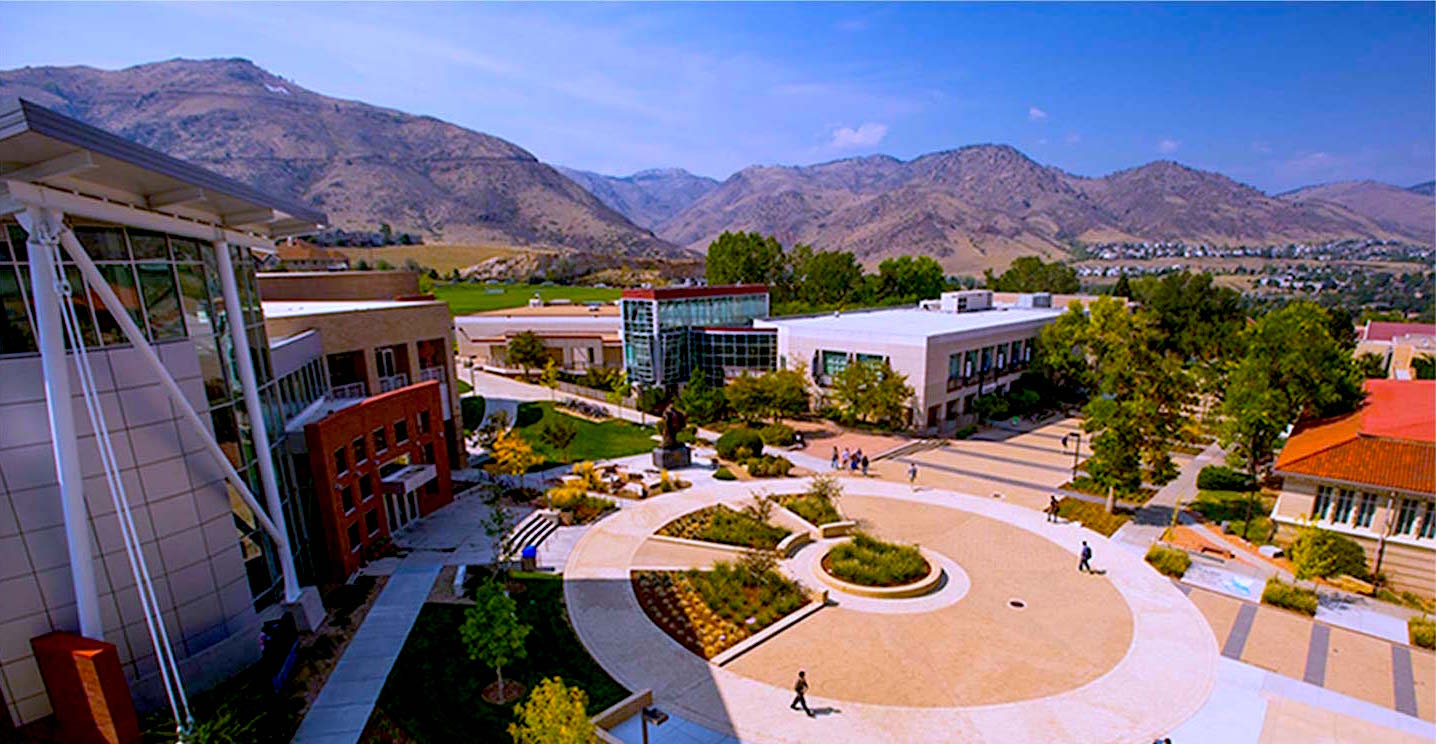
\includegraphics[width=2.5in]{Mines.jpeg}
\end{frame} %%%%%%%%%%%%%%%%%%%%%%%%%%
 
\begin{frame} %%%%%%%%%%%%%%%%%%%%%%%%%%
\frametitle{Instructor: Douglas Nychka}
\begin{minipage}{2.5in}
    \begin{itemize}
        \item  Professor at Mines, Director of the Data Science Program \vskip1em
        \item Ph.D., University of Wisconsin, Statistics, 1983 \vskip1em
        \item Focus: Curve and surface fitting, statistical computing \vskip1em
        \item Fellow ASA, IMS \vskip1em
        \item Senior Scientist Emeritus, National Center for Atmospheric Research
        \item Developer of the {\tt fields} and {\tt LatticeKrig} R  Packages
    \end{itemize}
\end{minipage}
\begin{minipage}{2in}
\centering
    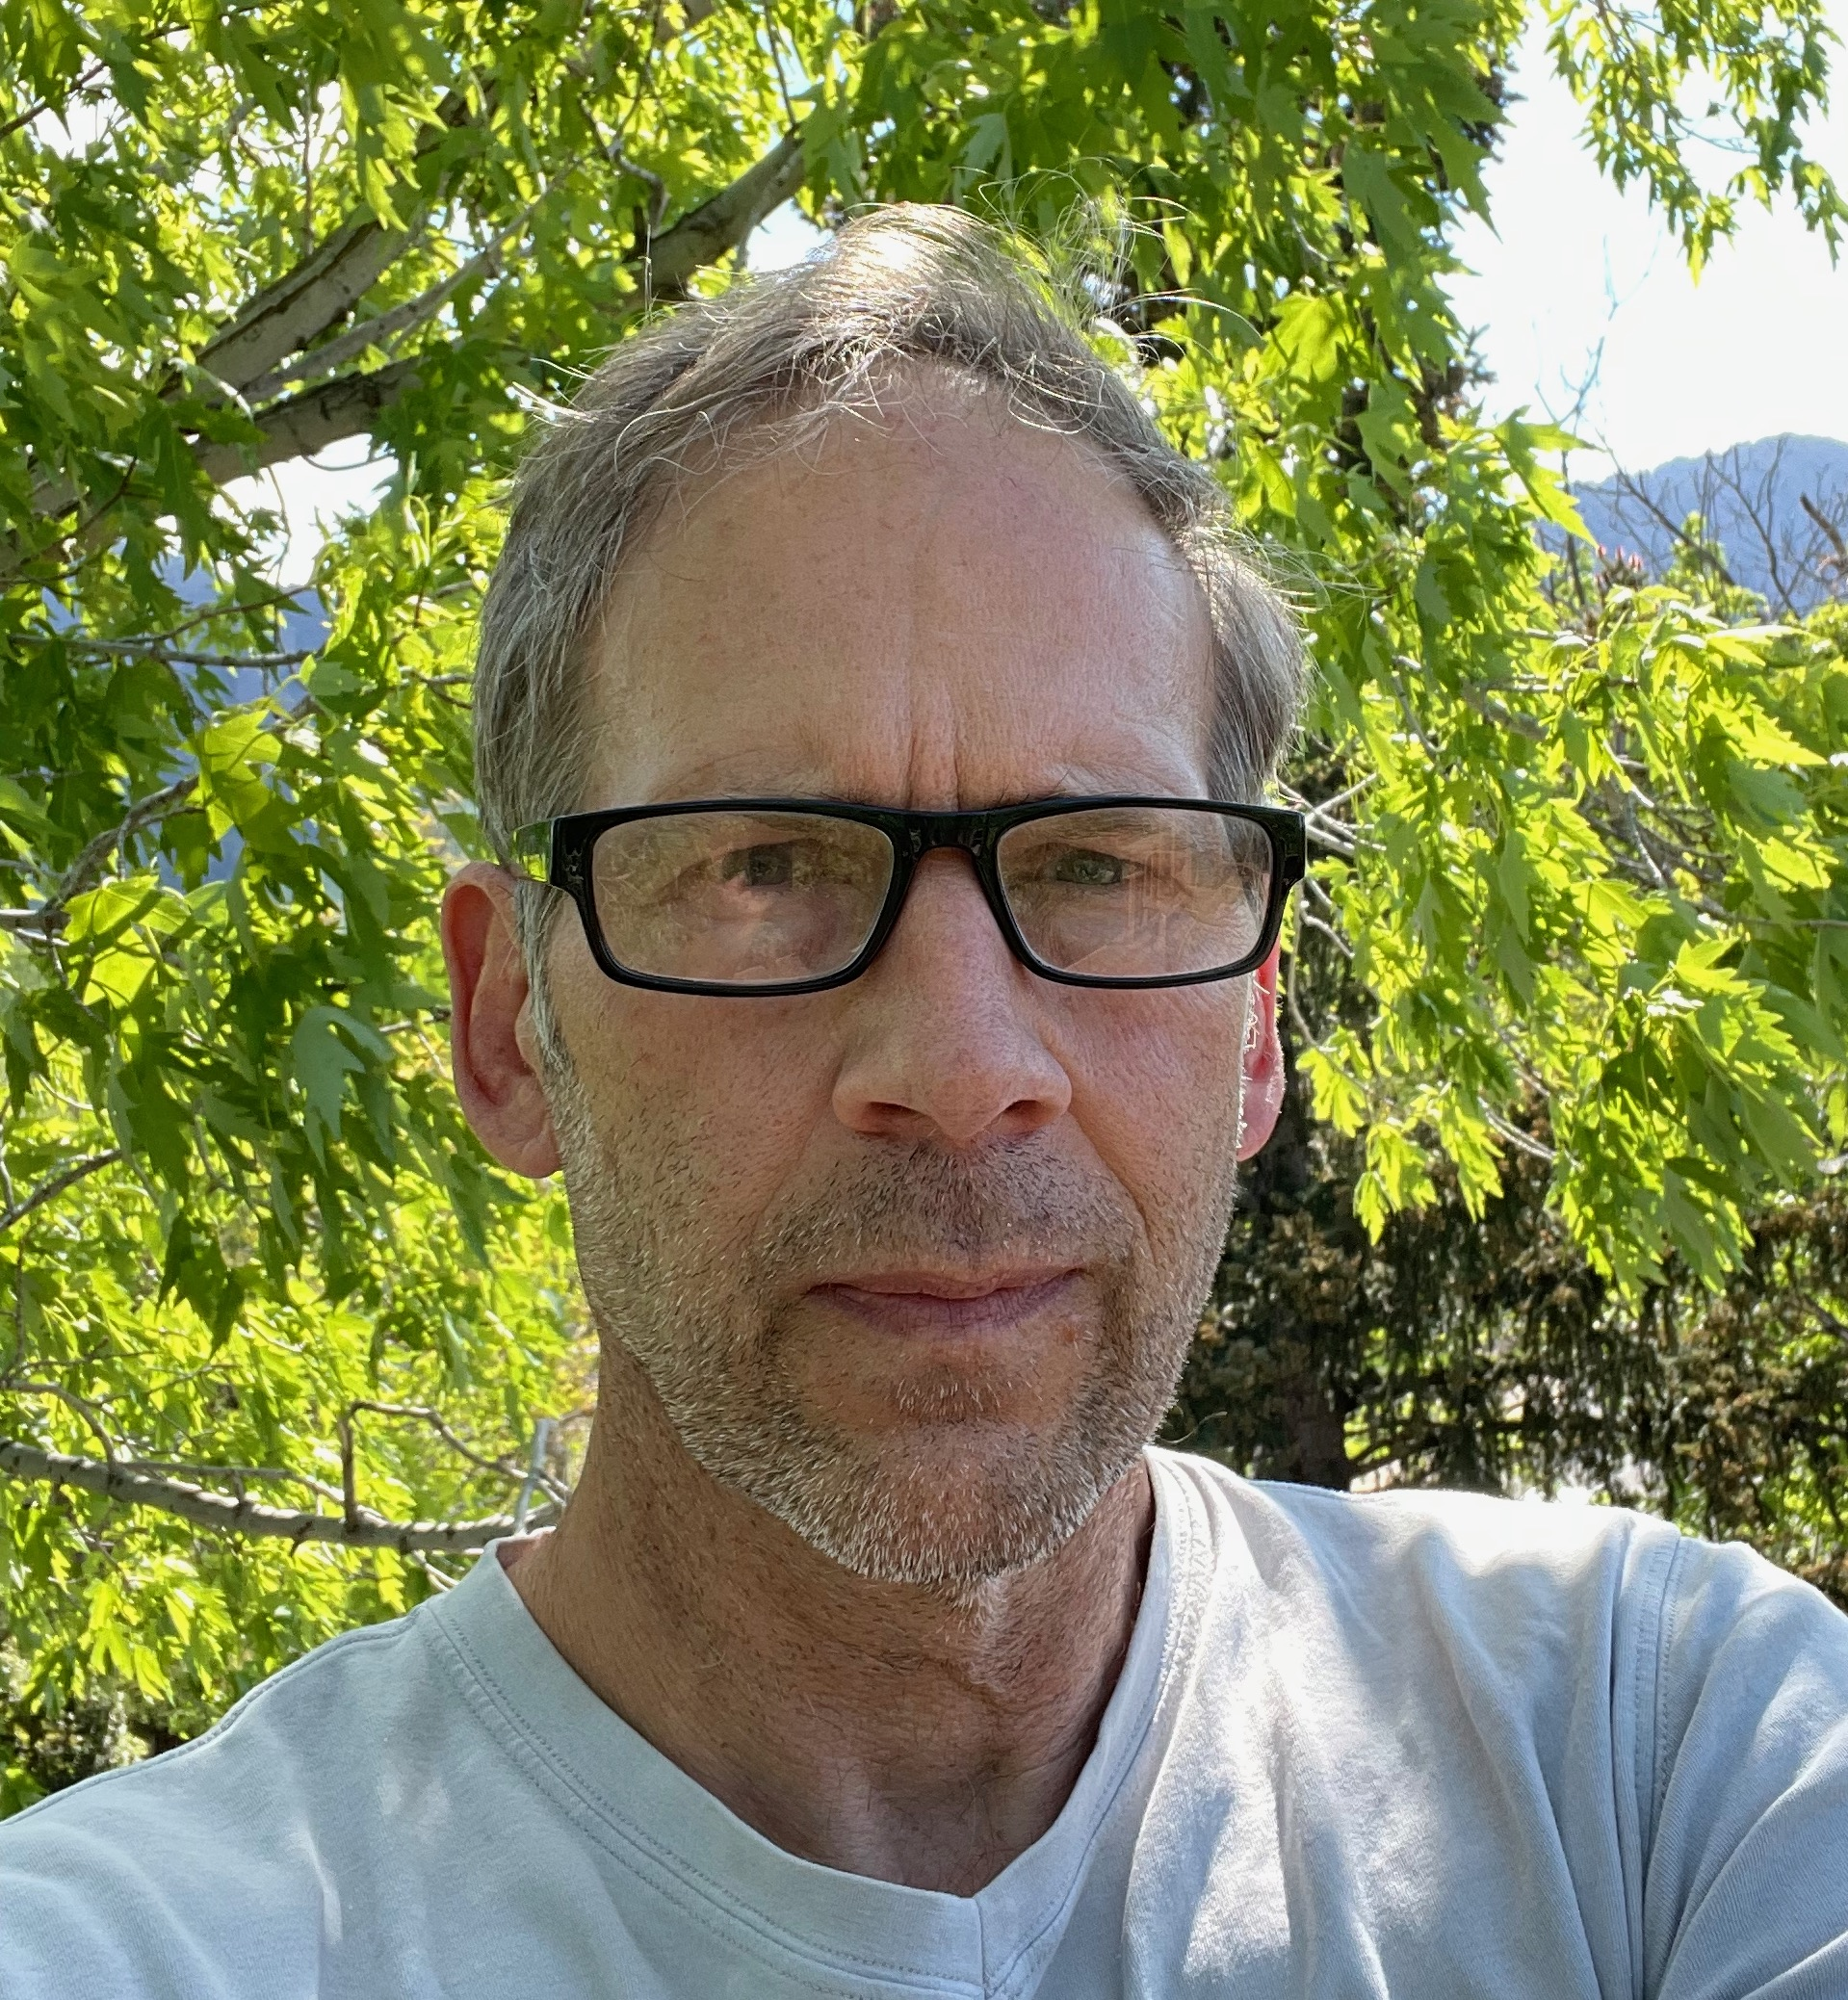
\includegraphics[height = 1.8in]{NychkaTrees.jpeg}
\end{minipage}
\end{frame} %%%%%%%%%%%%%%%%%%%%%%%%%%

\begin{frame} %%%%%%%%%%%%%%%%%%%%%%%%%%
\frametitle{Outline of the workshop}
\begin{itemize}
\item Module  1:  Large spatial data
\vskip2em
\item Module 2: Multivariate Spatial Data 
\vskip2em
\item Module 3: Dynamical models over space and time
\end{itemize}
\end{frame} %%%%%%%%%%%%%%%%%%%%%%%%%%

\begin{frame} %%%%%%%%%%%%%%%%%%%%%%%%%%
\frametitle{Outline}

Sections:
\begin{itemize}
\item   Large spatial data and linear algebra
\item  Representing curves with basis functions
\item  Fixed rank Kriging
\item  Spatial Autoregressions (SAR)
\item  LatticeKrig 

%\tableofcontents

\end{itemize}

\end{frame} %%%%%%%%%%%%%%%%%%%%%%%%%%
  
\section{Review of Kriging and timing}
%%%%%%%%%%%%%%%%%%%%%%%%%%
\begin{frame} %%%%%%%%%%%%%%%%%%%%%%%%%%
\frametitle{}
{\huge Part 1 Large spatial data and linear algebra}
\Myspace

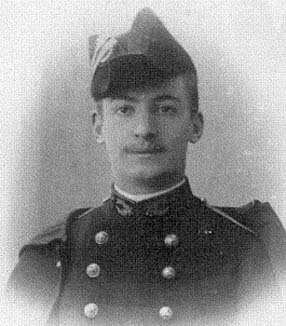
\includegraphics[width=1.5in]{pix/Andre_Cholesky.jpg} \ \includegraphics[width=1.25in]{../../../Current_talks/LKrigTalk/pix/DKrige.jpg} \\
A. Cholesky \hspace{1in} D. Krige

\end{frame} %%%%%%%%%%%%%%%%%%%%%%%%%%
%%%%%%%%%%%%%%%%%%%%%%%%%%

\begin{frame} %%%%%%%%%%%%%%%%%%%%%%%%%%
\frametitle{Recap of Kriging}
\begin{minipage}{3.5in}
\begin{itemize}
\item{\color{blue}\textbf{Recall:}}
$$
\begin{bmatrix}
\vspace*{0in}
\mathbf{X_1}\\
\cdots\\
\mathbf{X_2}
\end{bmatrix}
\sim
MN\left(
\overbrace{\begin{bmatrix}
\boldsymbol{\mu_1}\\
\cdots\\
\boldsymbol{\mu_2}
\end{bmatrix}}^{\boldsymbol{\mu}},
\overbrace{\begin{bmatrix}
\boldsymbol{\Sigma_{11}} & \boldsymbol{\Sigma_{12}}\\
\boldsymbol{\Sigma_{21}} & \boldsymbol{\Sigma_{22}}
\end{bmatrix}}^{\boldsymbol{\Sigma}}
\right)
$$
\item Suppose we observe $\mathbf{X_1}$ and want to predict $\mathbf{X_2}$.
\vskip2em
\item \[ \mathbf{X_2}|\mathbf{X_1}\sim MN(\boldsymbol{\mu_2}+\boldsymbol{\Sigma_{21}}
{\color{red} \boldsymbol{\Sigma_{11}}^{-1}}
(\mathbf{X_1}-\boldsymbol{\mu_1}), \boldsymbol{\Sigma_{22}}-\boldsymbol{\Sigma_{21}}
{\color{red} \boldsymbol{\Sigma_{11}}^{-1}}
\boldsymbol{\Sigma_{12}}) \]
\end{itemize}
\end{minipage}
\ 
\begin{minipage}{.75in}
\vspace*{0in}
\includegraphics[width=.5in]{../../../Current_talks/LKrigTalk/pix/DKrige.jpg} \\
D. Krige
\end{minipage}

\end{frame} %%%%%%%%%%%%%%%%%%%%%%%%%%

 \begin{frame} %%%%%%%%%%%%%%%%%%%%%%%%%%
 \frametitle{Computing these expressions}
\bdot ${\color{red} \boldsymbol{\Sigma_{11} } }$ : 
the covariance matrix for the observations.  \\
If there are 1000 observations, this matrix is $1000 \times 1000$.  \\
\Myspace
\bdot To find MLEs also need the determinant of $\Sigma_{11}$.  \\
\Myspace
Computing expressions with {\color{red} $ \Sigma_{11}^{-1}$} and {\color{red} $ | \Sigma_{11}| $} grow as the cube of the number of observations. \\
\Myspace
\Myspace
 Twice as many observations will take  $8= 2^3 $ times longer. 
\end{frame} %%%%%%%%%%%%%%%%%%%%%%%%%%

\begin{frame} %%%%%%%%%%%%%%%%%%%%%%%%%%
 \frametitle{Its all about the Cholesky}
 {\it For the linear algebra fans ... } \\
 Spatial statistics computations make heavy use of the Cholesky decomposition.  \\
\bdot  $A$ a positive definite, symmetric matrix \\
{\it Cholesky decomposition} is  $A= LL\T$ where $L$  is a {\it lower triangular} matrix. \\
\Myspace
\bdot Compute  $\by \T A^{-1}  \by$  by 
\[ \by \T A^{-1}  \by = \by \T (L L\T) ^{-1}  \by  = ( L ^{-1} \by) \T  (L ^{-1} \by)
=  \bw \T \bw \]
 $\bw$ {\it solves }  the linear system $L   \bw = \by $.  \\
{\it Solving a  triangular system  is  very efficient.} \\
\Myspace
\bdot Compute determinant $A$. \[ |A| =  |L L\T | =  |L | | L\T | = |L|^2 \]
The determinant of a  triangular matrix is the product of the diagonal elements. 
\end{frame} %%%%%%%%%%%%%%%%%%%%%%%%%%

\begin{frame} %%%%%%%%%%%%%%%%%%%%%%%%%%
\frametitle{Sparse matrices}
\bdot  $A$ is sparse if it has many zeros  \\
  (Typically we want the number of non-zero elements to grow  linearly with the number of dimensions. ) \\
  \Myspace
  \bdot If $A$ is sparse to find  $Ax$  skip over the zero elements to speedup multiplication  \\
    \Myspace
 \bdot If $A$ is sparse  Cholesky decomposition can also be sparse this will speed up solving linear systems.

\end{frame}  

\begin{frame} %%%%%%%%%%%%%%%%%%%%%%%%%%
\frametitle{More on Sparse matrices}
 A banded matrix with its Cholesky decomposition   $A= LL^T$
 {\small
 \[   A= \left[
     \begin{array}{rrrrr}
      9 & -3 & 0& 0&0 \\
       -3 &10&  -3& 0&0 \\
       0&-3 &10&  -3& 0\\
        0&0&-3 &10&  -3\\
         0& 0&0&-3 &10\\
         \end{array}
         \right]
         \mbox{ and }
          L= \left[
           \begin{array}{rrrrr}
      3 & 0 & 0& 0&0 \\
       -1 &3& 0& 0&0 \\
       0&-1 &3& 0& 0\\
        0&0&-1 &3& 0\\
         0& 0&0&-1 &3\
         \end{array}
          \right]  
     \]  
     } % end font  
     
     
\bdot With $L$ triangular and sparse very fast to  evaluate/ solve for  $L^{-1} x$. \\

This means it is fast to evaluate. 
\[ x^TA^{-1}x  = (L^{-1}x )^T L^{-1} x  \mbox{ and }  |A| = |L | |L^T| =  |L|^2 \] 

     
\end{frame}
 
\begin{frame} %%%%%%%%%%%%%%%%%%%%%%%%%%
\frametitle{More on Sparse matrices}     
Order matters:
{\small 
\[
A =  \left[ \begin{array}{rrrrr}
      x & 0 & 0& 0 &x \\
       0&x& 0& 0 & x \\
       0&0&x& 0 & x\\
        0&0&0 &x & x\\
         x& x& x& x & x 
         \end{array}
          \right]
           \mbox{ factors as  }
           L=  \left[ 
      \begin{array}{rrrrr}
      x & 0 & 0& 0&0 \\
       0&x& 0& 0&0 \\
       0&0&x& 0& 0\\
        0&0&0 &x& 0\\
         x& x&x&x &x \
         \end{array}
          \right]       
     \] 
     But  
     \[
A =  \left[ \begin{array}{rrrrr}
      x & x& x& x & x \\
       x&x& 0& 0 & 0 \\
       x&0&x& 0 & 0 \\
        x&0&0 &x & 0 \\
         x& 0& 0& 0 & x 
         \end{array}
          \right]
           \mbox{ factors as  }
           L=  \left[ 
      \begin{array}{rrrrr}
      x & 0 & 0& 0&0 \\
       x&x& 0& 0&0 \\
       x&x&x& 0& 0\\
        x&x&x &x& 0\\
         x& x&x&x &x \
         \end{array}
          \right]       
     \] 

}

\bdot Permute rows and columns of $A$ to increase sparsity. \\
E.g. {\color{blue} AMD } is an ordering  algorithm to find  approximate minimum degree of a sparse matrix 
 \end{frame}
 
\begin{frame} %%%%%%%%%%%%%%%%%%%%%%%%%%
\frametitle{Our strategy} 

  {\large Formulate statistical models for spatial data that lead to sparse linear algebra. }
 
 \end{frame}

%\begin{frame} %%%%%%%%%%%%%%%%%%%%%%%%%%
% \frametitle{Dodging an inverse}
 
% \end{frame}

\section{Basis functions}
%%%%%%%%%%%%%%%%%%%%%%%%%%
\begin{frame} %%%%%%%%%%%%%%%%%%%%%%%%%%
\frametitle{}
{\huge  Part 2 Basis functions for curve fitting}
\Myspace
\hspace*{.25in} 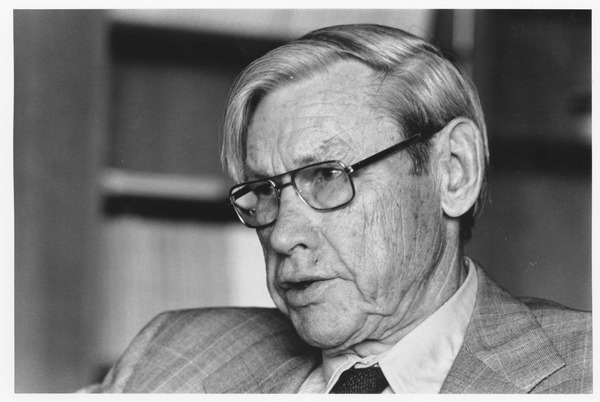
\includegraphics[width=1.25in]{pix/stone.jpg} 
\ 
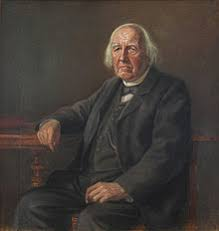
\includegraphics[width=1in]{pix/weierstrauss.jpeg} \\
\hspace*{.35in} M. Stone \hspace{.6in}  K. Weierstrauss \\
\Myspace
\Myspace

\includegraphics[width=3in]{../../../Current_talks/LKrigTalk/pix/sandPile6.pdf}

\end{frame}   %%%%%%%%%%%%%%%%%%%%%%%%%%
%%%%%%%%%%%%%%%%%%%%%%%%%%

\begin{frame} %%%%%%%%%%%%%%%%%%%%%%%%%%
\frametitle{Representing a curve}
Start with your favorite 
$m$ basis functions $\{b_1(s), b_2(s), \ldots, b_m(s)\}$

The curve  has the form 

\Mycomment{
\[{g}(s)=\sum_{k=1}^{m}b_{k}(s){c}_{k}\]}
where
${\bc}=({c}_1, \ldots, {c}_m)$ are the coefficients.
\\
\Myspace
\bdot The basis functions are fixed \\
\bdot Based on data  find the coefficients.  \\
\bdot $m$ does not have to be the same as the number of observations. 
\\
\Myspace
Many spatial statistics problems have this general form or can be approximated by it.

\end{frame} %%%%%%%%%%%%%%%%%%%%%%%%%% 

\begin{frame} %%%%%%%%%%%%%%%%%%%%%%%%%%
\frametitle{Example of basis functions}

\includegraphics[height=2in]{/Users/nychka/Home/Current_talks/KAUST/pix/bumpShape.pdf}

\bdot Build a basis by translating and scaling a bump shaped curve

\bdot Not your usual sine/cosine or polynomials!

\bdot Bsplines not required!

\end{frame} %%%%%%%%%%%%%%%%%%%%%%%%%%


 \begin{frame} %%%%%%%%%%%%%%%%%%%%%%%%%%
 \frametitle{Two Bases}

10 Functions: \\
\includegraphics[height=1in]{/Users/nychka/Home/Current_talks/KAUST/pix/bumpBasisA.pdf} \\
20 Functions: \\
\includegraphics[height=1in]{/Users/nychka/Home/Current_talks/KAUST/pix/bumpBasisB.pdf}

Use both together  ( $10+20 = 30$ functions) to represent two different scales of detail.

\end{frame} %%%%%%%%%%%%%%%%%%%%%%%%%%

\begin{frame} %%%%%%%%%%%%%%%%%%%%%%%%%%
 \frametitle{In two dimensions}
 \includegraphics[height=.75in]{/Users/nychka/Home/Current_talks/LKrigTalk/pix/sandPile8.pdf} \hspace{.5in}
  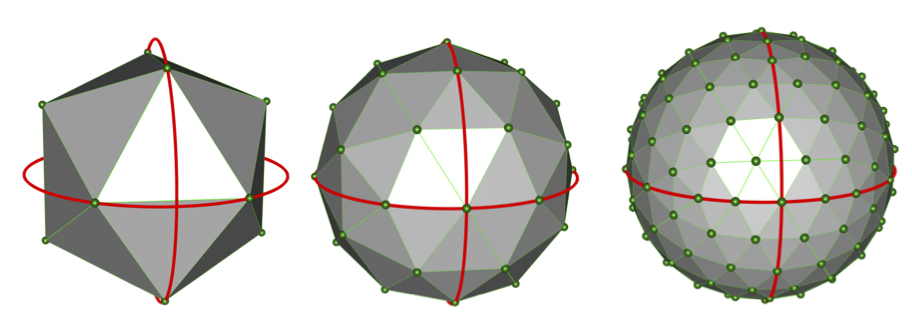
\includegraphics[height=.75in]{/Users/nychka/Dropbox/Home/Teaching/ISIShortCourse/LargeSpatialData/pix/balls.jpg}
 \\
 Example of a 2-d bump   \hspace{1in} Lattice on a sphere  \\
 
 \Myspace
 \Myspace
 Defining the bump
 \[ b(\bs) =  \Phi( \| \bs - \bu \|/ \alpha )  \]
 $\Phi$  a fixed bump shaped function, $\bu$ the knot, and $\alpha$ is a scale factor.  \\
 
 \bdot    Gaussian,  $ \Phi(d) = e^{-d^2}$  \\
% \bdot    Biweight,  $(1- d)^2 $   for $(d <1 )$  zero otherwise,   \\
 \bdot    Wendland  (2,2),  \[ \Phi(d) = (1- d)^6 ( 35d^2 + 18d  +3)/ 3  \quad (d \le 1 )  \mbox{ zero otherwise }  \]  

 \end{frame} %%%%%%%%%%%%%%%%%%%%%%%%%%

\begin{frame} %%%%%%%%%%%%%%%%%%%%%%%%%%
\frametitle{
Basis function matrix }

The {\it basis matrix}: 
\[X_{i,k} = b_k(\bs_i)\] 
rows index locations, columns index the basis functions. \\
\Myspace
%$( \hat{g}(s_1), \hat{g}(s_2), \ldots, \hat{g}(s_n) )^T =X {\bc} $
 and  so
 
 \[\bg = X{\bc}  \]

\bdot If  the basis functions have compact range then $X$ is sparse. \\
\Myspace
\bdot  If $X$ is sparse then so will  $X^TX$ .


\end{frame} %%%%%%%%%%%%%%%%%%%%%%%%%%



\section{Fixed Rank Kriging}
%%%%%%%%%%%%%%%%%%%%%%%%%%
\begin{frame} %%%%%%%%%%%%%%%%%%%%%%%%%%
\frametitle{}
{\huge Part 3  Fixed Rank Kriging} \\
\Myspace
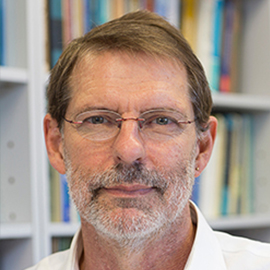
\includegraphics[width=1.5in]{pix/cressie.jpg}

See: N. Cressie and G. Johannesson. (2008) 

\end{frame} 
%%%%%%%%%%%%%%%%%%%%%%%%%%
%%%%%%%%%%%%%%%%%%%%%%%%%%


\begin{frame} %%%%%%%%%%%%%%%%%%%%%%%%%%
\frametitle{A model for the coefficients}
{\large
\[ g(s) =  \sum_k b_k(s) c_k  \mbox{ and }  \bc \sim N( 0, \Omega) \]
\Myspace
$g(s)$ is a now a spatial process because $\bc$ is a random vector.
}
\end{frame} %%%%%%%%%%%%%%%%%%%%%%%%%%



\begin{frame} %%%%%%%%%%%%%%%%%%%%%%%%%%
\frametitle{More about this random effects model}
Suppose:  \\
\Myspace
\bdot Basis functions are bumps centered at the knots $u_1, u_2, \ldots u_m$  \\
\Myspace
\bdot Use a spatial covariance to model dependence among coefficients using knot locations. \\
\Myspace
\Mycomment{An Example of $\Omega$ } 
\[ Cov( c_k, c_k ) = \Omega_{k,k} =  e^{ -| u_k - u_k |/ \alpha } \]

\[ g(s) =  \sum_k b_k(s) c_k \]
is now a {\it random} curve. 
\end{frame} %%%%%%%%%%%%%%%%%%%%%%%%%%


\begin{frame} %%%%%%%%%%%%%%%%%%%%%%%%%%
\frametitle{The covariance function}

Using linear statistics: 
\[ Cov( g(s), g(s^{\prime} ) =  \sum_{j,k}  b_j(s) b_k(s^{\prime}) \Omega_{j,k} \]

The covariance matrix for $g$ at the observations has the simple  formula  \\
\[ X \Omega X\T \]

\end{frame} %%%%%%%%%%%%%%%%%%%%%%%%%%

\begin{frame} %%%%%%%%%%%%%%%%%%%%%%%%%%
\frametitle{An example}
Ten  Wendland basis function  scale of .4, exponential covariance with range .2. \\
\Myspace
\Myspace
\begin{tabular}{ccc}
Covariance of $\bc$ & Covariance of $g(s)$ & Precision of $\bc$ \\
 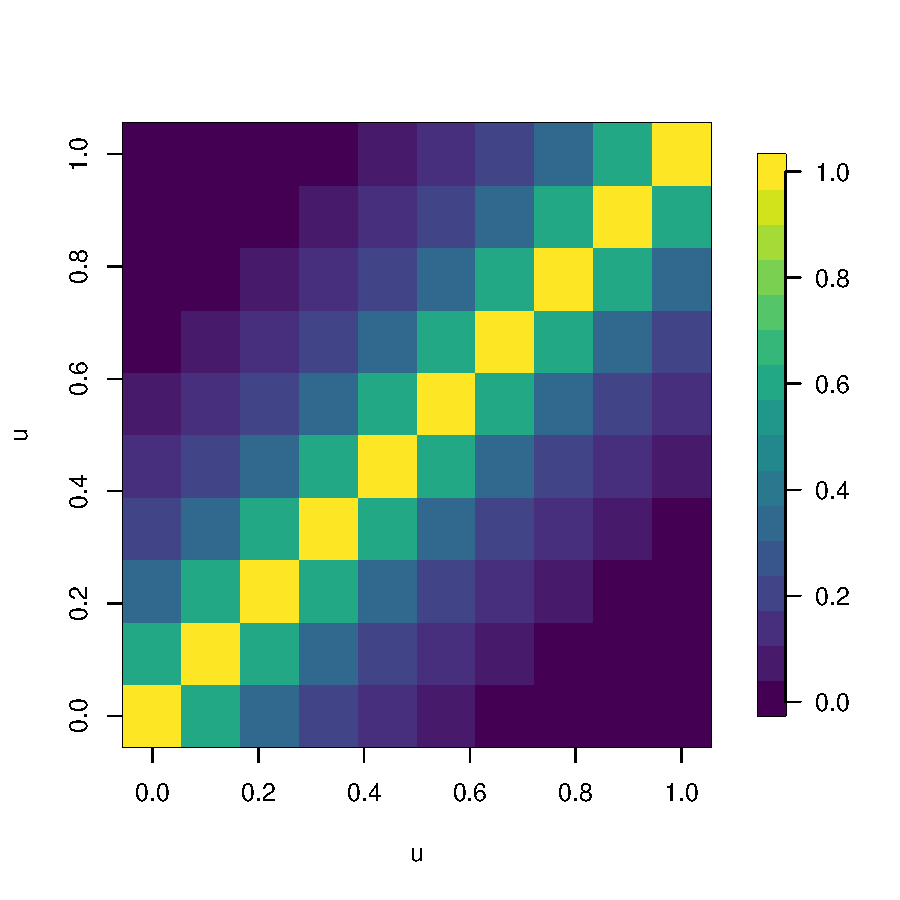
\includegraphics[height=.75in]{pix/FRKCovCoef.pdf} & 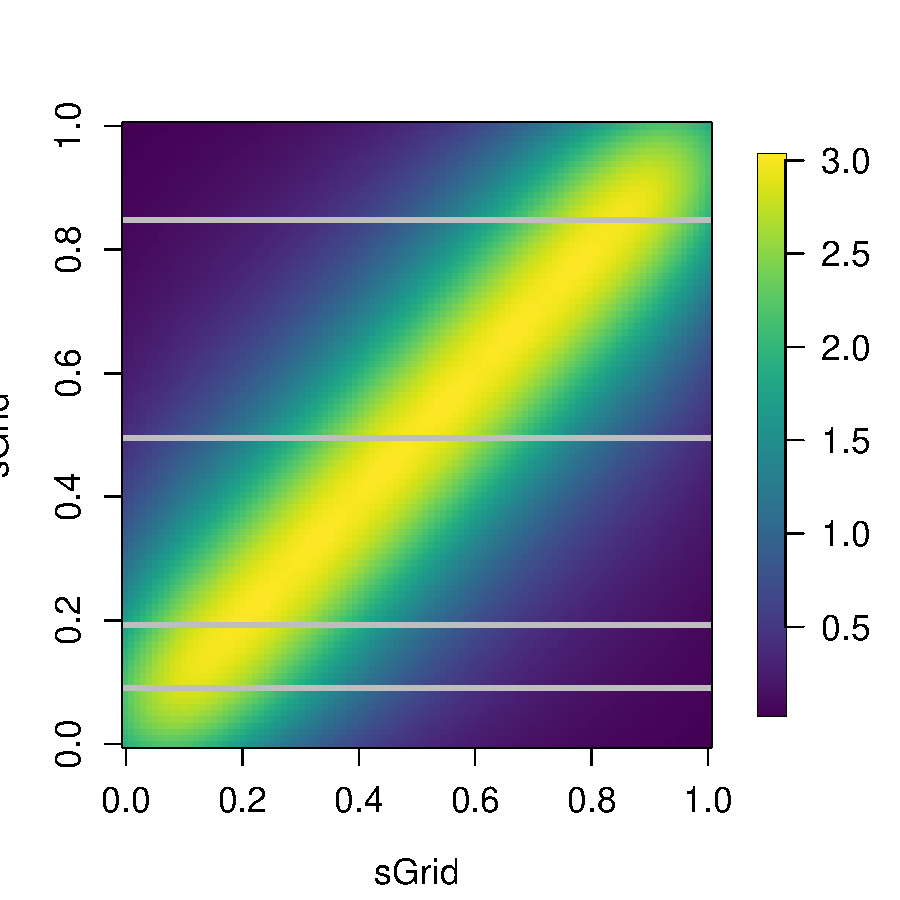
\includegraphics[height=.75in]{pix/FRKCovImage.pdf} &
 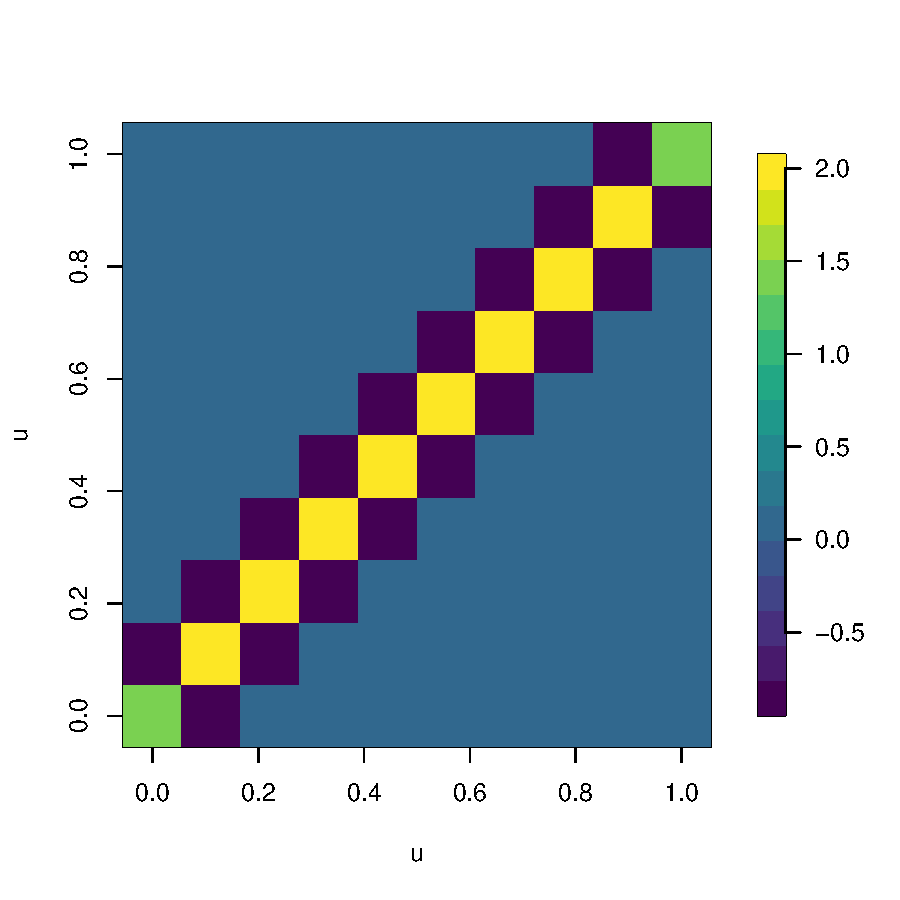
\includegraphics[height=.75in]{pix/FRKPrecisionCoef.pdf} 
 \end{tabular}\\
Four slices of  the  $g(s)$ covariance matrix \\
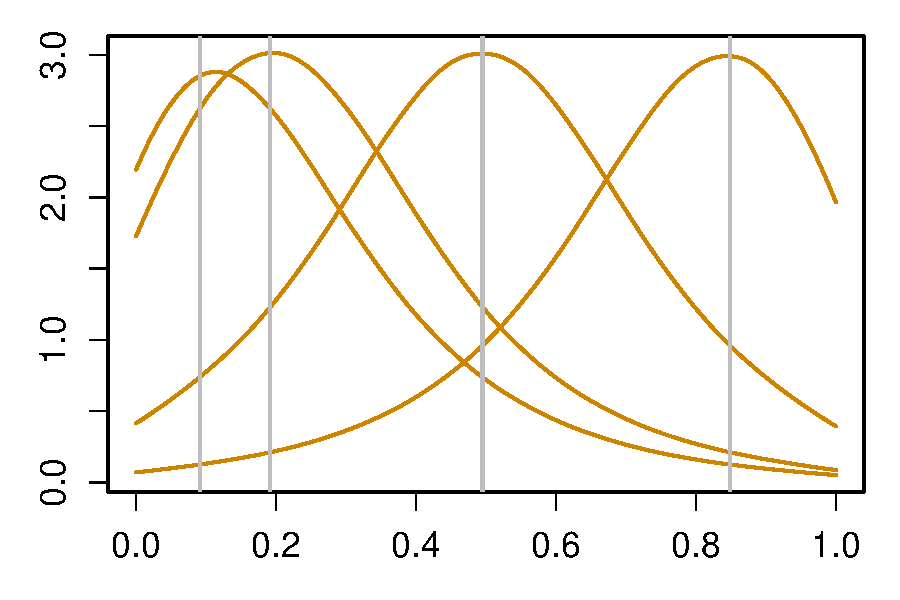
\includegraphics[height=1in]{pix/FRKCov.pdf}
 \\
Hard to the see the 10 RBFs!  Looks a lot like a Matern,  smoothness =1. 
 
\end{frame} %%%%%%%%%%%%%%%%%%%%%%%%%%

\begin{frame} %%%%%%%%%%%%%%%%%%%%%%%%%%
\frametitle{Estimating the coefficients }
\Mycomment{Basic idea: find $\bc$ given $\by$} \\
\Myspace
\Myspace
Based on the multivariate normal or BLUE, 
\[ \hat{{c}} = ( X^T X  +  \Omega^{-1} ) ^{-1} X^T \by \]
or 
\[  ( X^T X  +  \Omega^{-1} ) \hat{{c}} = X^T \by \]

\bdot This is  fixed rank Kriging. \\
\bdot  Also known as ridge regression estimate.  \\
\Myspace
\bdot Better to work directly with the inverse of $\Omega$,   $Q= \Omega^{-1}$ \\
\Myspace   
\bdot Compute using the Cholesky! \\
\Myspace 
{\color{red} If $X$ is sparse and $\Omega^{-1}$ is sparse then this is now a sparse linear
 algebra problem.}

\end{frame} %%%%%%%%%%%%%%%%%%%%%%%%%%

\section{Spatial Autoregressions}
%%%%%%%%%%%%%%%%%%%%%%%%%%
\begin{frame} %%%%%%%%%%%%%%%%%%%%%%%%%%
\frametitle{}
{\huge Part 4 \\
 Spatial Autoregessions (SARs)}
 \Myspace
 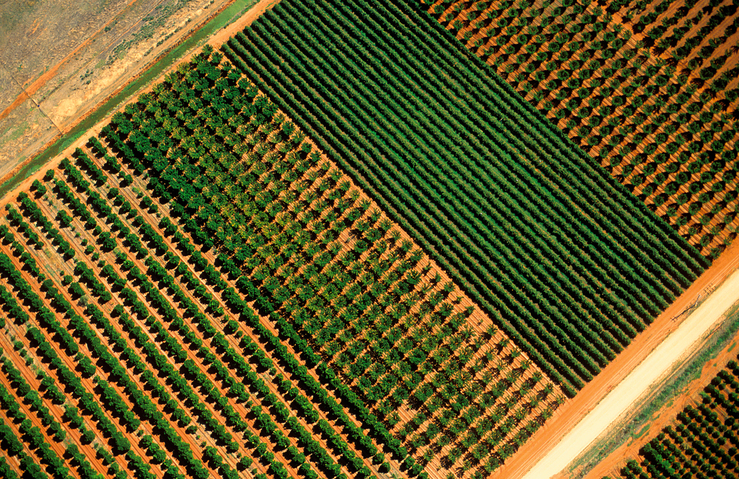
\includegraphics[width=3in]{pix/orchard.jpg}

\end{frame} %%%%%%%%%%%%%%%%%%%%%%%%%%
%%%%%%%%%%%%%%%%%%%%%%%%%%

\begin{frame} %%%%%%%%%%%%%%%%%%%%%%%%%%
\frametitle{ SAR models for $\bc$}
A 1-D case \\
\Myspace
\begin{minipage}{2in}
 \Mycomment{Some coefficients:  } \\
   \begin{tabular}{ccccccc}
.& $c_{k-2}$&$c_{k-1}$ &  {\color{red4} $c_{k}$} &$c_{k+1}$ &$c_{k+2}$ &.\\
\end{tabular}
\end{minipage}
\\
\Myspace
\begin{minipage}{2in}
 \Mycomment{Some weights:  } \\
   \begin{tabular}{ccccccc}
0& 0 &$ -1$ &  {\color{red4} {\tt a}} & $-1$&0&0 \\
\end{tabular}
\end{minipage}
\\
\Myspace
\Mycomment{A spatial autoregression:}  
\\
\[   {\color{red4} {\tt a}}  c_k  -  ( c_{k-1} + c_{k+1} )  = {\color{red4} {\tt a}}  c_k  -  c_{k-1} - c_{k+1}   =  e_k \]
$ \{ e_k \}$  are iid $N(0,1) $ 
\end{frame}

\begin{frame} %%%%%%%%%%%%%%%%%%%%%%%%%%
\frametitle{Combining coefficients}
\[ B \bc = \be \]
where $\be \sim N( 0, I) $
\\
$\bB$ a matrix where each row has 3 nonzero weights:  \\
a  diagonal element, $a$ and  two  
first order neighbors ($-1$).  
\\
\Myspace
\bdot ${\color{red4}  {\tt a} }$ parameter needs to be greater than 2  \\
\bdot  Precision matrix $Q =  B^T B $ , this is $\Omega^{-1}$! \\
\bdot Covariance matrix for $\bc$ is  $ \Omega =  Q^{-1}  =  B^{-1} $ \\
\bdot $B$ and $Q$ are sparse matrices.  \\
\Myspace 
NOTE: For practical use the variance  and correlation range of this process is related to $a$ and it is useful to normalize to a fixed variance. 
\end{frame}

\begin{frame} %%%%%%%%%%%%%%%%%%%%%%%%%%
\frametitle{SAR in two dimensions}
\begin{minipage}{2in}
 \Mycomment{Some coefficients:  } \\
 {\large
   \begin{tabular}{ccccc}
 .&.&.& .&.\\
.&. & $c_{j-1,k}$ & . &.\\
.&$c_{j,k-1}$ &  {\color{red4} $c_{j,k}$} & $c_{j, k+1}$&. \\
.&.& $c_{j+1,k}$ & . &. \\ 
 .&.&.&.&.\\
\end{tabular}
}
\end{minipage}
\hspace{.5in}
\begin{minipage}{2in}
 \Mycomment{Some weights:  } \\
 {\large
   \begin{tabular}{ccccc}
 .&.&.& .&.\\
.&. & -1 & . &.\\
.&-1 &  {\color{red4} {\tt a}}  & -1&. \\
.&.& -1 & . &. \\ 
 .&.&.&.&.\\
\end{tabular}
}
\end{minipage}
\\
\Myspace
\bdot Same concept although indexing is more difficult \\
\bdot  $B$ is a sparse matrix with  5 nonzero elements on each row.  \\
\bdot $a$ must be greater than 4. 
\end{frame}



\section{LatticeKrig Model and Package}
%%%%%%%%%%%%%%%%%%%%%%%%%%
\begin{frame} %%%%%%%%%%%%%%%%%%%%%%%%%%
\frametitle{}
{\huge Part 5 
{\it LatticeKrig}
 }\\
 \Myspace
 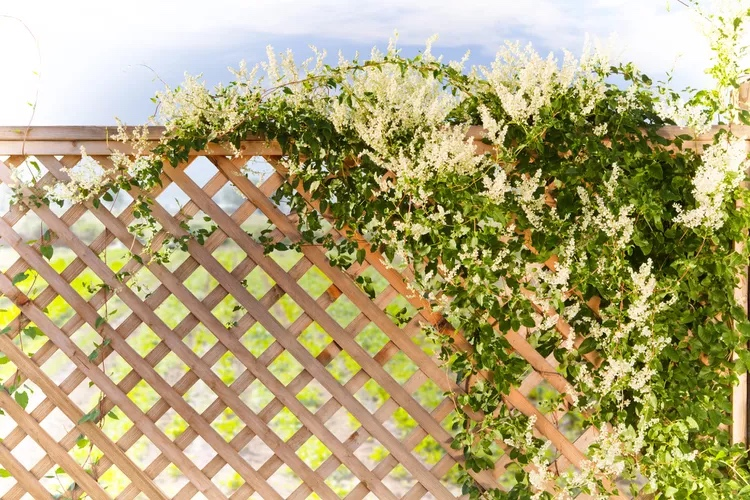
\includegraphics[width=3in]{pix/garden-lattice.jpeg}

 
\end{frame} %%%%%%%%%%%%%%%%%%%%%%%%%%
%%%%%%%%%%%%%%%%%%%%%%%%%%

\begin{frame} %%%%%%%%%%%%%%%%%%%%%%%%%%
\frametitle{LatticeKrig model}

A  specific, Fixed Rank Kriging model 

\begin{enumerate}
 
\item  Basis functions at regular knots and compact support (zero beyond fixed range). 
    Use the Wendland function. \includegraphics[height=.35in]{/Users/nychka/Home/Current_talks/LKrigTalk/pix/sandPile8.pdf} 
      \\
     \Myspace
     \ 
  
\item Coefficients follow a SAR model \\
-- for first or second order neighbors. 
  {\tiny \begin{tabular}{ccccc}
 .&.&.& .&.\\
.&. & -1 & . &.\\
.&-1 &  {\color{red4} {\tt a}}  & -1&. \\
.&.& -1 & . &. \\ 
 .&.&.&.&.\\
\end{tabular}
}
  \\
     \Myspace
     \ 
\item  $\hat{\bc}$ found by  Kriging   $( X^T X  +  \Omega^{-1} ) \hat{{c}} = X^T \by$

\end{enumerate}
\Myspace
\Mycomment{Why all this trouble?} \\

{\color{red} Basis functions and SAR model give sparse matrices} \\

\end{frame} %%%%%%%%%%%%%%%%%%%%%%%%%%

\begin{frame} %%%%%%%%%%%%%%%%%%%%%%%%%%

\frametitle{Some practical additions}

The Lattice Krig model should give reasonable covariance functions and follow standard Kriging results.  \\
\Myspace
\bdot Add a linear function to the basis. \\
\Myspace
\bdot Add several different scales of basis functions  together to  approximate standard covariance functions.  \\
\Myspace
\bdot Normalize the SAR/basis functions to give a process with a unit variance  \\
\Myspace
\end{frame}%%%%%%%%%%%%%%%%%%%%%%%%%%

\begin{frame} %%%%%%%%%%%%%%%%%%%%%%%%%%

\frametitle{}
\Mycomment{Parameters in the model }
 \[ \by_i = g( \bs_i) + \epsilon_i \]
 \bdot $Var( g(\bs_i) ) = \sigma^2$\\
 \bdot $Var( \epsilon_i ) = \tau^2$ \\
 \Myspace 
 \bdot {\color{red} $a$ } parameter in  the SAR   \\
 \bdot  {\tt NC} Number of basis functions in each dimension \\
 
 \bdot {\tt nlevel} Number of multiresolution levels.  \\
 \bdot {\tt nu} Smoothness  \\
 \Myspace
 {\tt NC} chosen based on resolution of $g$ \\
 {\tt nlevel} as large as possible ( $\sim$ 3). \\
 {\tt nu} tracks the Matern interpretation, is hard to estimate  from data and is also specified. 
%

\end{frame}%%%%%%%%%%%%%%%%%%%%%%%%%%



\section{Summary}


\begin{frame} %%%%%%%%%%%%%%%%%%%%%%%%%%
\frametitle{Summary}
\begin{itemize}
\item Standard Kriging model breaks down with large data. 
\item An approximate model can be used based on basis functions and random coefficients
\item Choosing compact basis functions and a SAR lead to sparse matrices and fast computation.
\item The LatticeKrig model can be tuned to approximate standard Kriging results but for large data sets. 
\end{itemize}
\end{frame}%%%%%%%%%%%%%%%%%%%%%%%%%%
\begin{frame} %%%%%%%%%%%%%%%%%%%%%%%%%%
\frametitle{Thanks!}
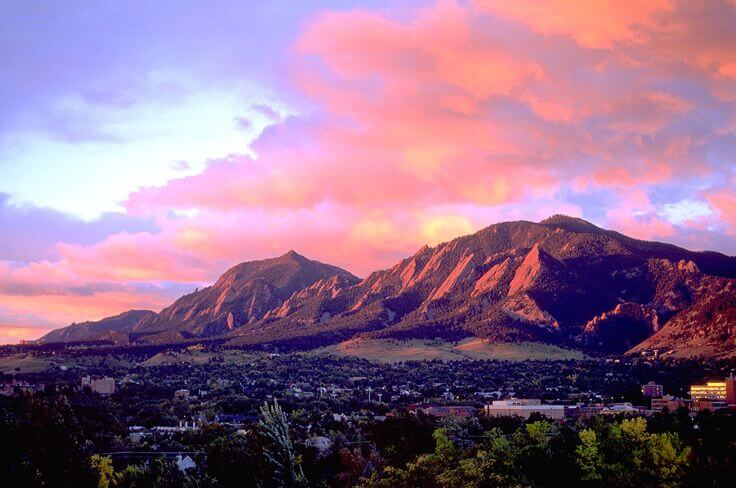
\includegraphics[width=3in]{pix/flatirons.jpeg}
\end{frame}

\end{document}